\hypertarget{Edge Intelligence}{%
	\chapter{Edge Intelligence}\label{ch:edgeintelligence}}
\thispagestyle{fancy}

\acrlong{ei} is artificial intelligence application and services deployed at the edge of the network. The primary objective of \gls{ei} is to enable \gls{ai} for mobile and \gls{iot} application. Progress within \gls{ml} have been pushed by the achievements within \gls{cv} and \gls{nlp} using \gls{dnn}s. However deployment of \gls{dnn} in real applications have been limited to the cloud, as state-of-the-art \gls{dnn} have been too computationally expensive to run elsewhere. The improvement have mostly been impacted by efforts in training deeper models with the ability to learn increasingly complex features. The tendency is exemplified by the winner of ImageNet Challenge \cite{russakovsky_imagenet_2015}; within a time span of only four years, have the number of layers have grown from 8 to 152 layers. 

Increasing deeper model have hindered deployment of intelligent services onto mobile and \gls{iot} devices, which have made cloud intelligence inevitable. Running algorithm in large-scale data centers comes with the side-effect of introducing unpredictable communication delays, caused by congestions in shared communication medium and shared computing resources in the data center. The added delay from cloud intelligence have made real-time \gls{ai} impractical for mobile and \gls{iot} devices. Although end-devices have become more powerful in recent years, more lightweight albeit less accurate \gls{dnn} architectures have been proposed. Deployment of state-of-the-art \gls{dnn}s on edge server aims at reducing inference latency, energy consumption and memory footprint by offloading the heavy task from the end-device onto edge servers, without introducing the communication latency bottleneck by running state-of-the-art algorithm in the cloud. 


Edge intelligence is a promising compromise to obtain state-of-the-art performance in real-time, necessary for applications such as \gls{ar}/\gls{vr}, \gls{av} and Personal Assistant with very stringent latency and reliability requirements. In edge computing data processing is done in closer proximity to end-users, the shortened communication path leads to a reduction in communication latency. Edge computing seeks to distibute computing resources in sharp contrast to the last decade of centralization of computing resources for cloud computing \cite{shi_edge_2016}. Edge computing is envisioned to reliably serve the ever growing number of billions upon billions of connected mobile and \gls{iot} devices. By 2020 Cisco Internet Business Solutions Group, 50 billion things is predicted to be connected to the internet. The amount of data generated by mobile and \gls{iot} device at the edge of the network is expected to overwhelm cloud data centers and exhaust available bandwidth. Hence edge computing is a possible and probably a necessary step in the development and democratizing of \gls{ai}.

Research have shown, that the conventional cloud-only approach in many cases is actually slower than a mobile-only execution in \cite{kang_neurosurgeon:_2017}, as mobile devices are getting more resourceful and nowadays it is not uncommon to have a smartphone equipped with a \gls{gpu}. To avoid draining the battery \gls{iot} devices, it may not be desired to run heavy \gls{ai} algorithms, which makes remote offloading a necessity.  In \cite{karlsen_prototyping_nodate} edge-based offloading are investigated and show significant latency improvement compared to both device- and cloud intelligence by offloading \gls{ai} tasks from \gls{cpu}-enabled end devices to a \gls{gpu}-enabled edge server. 

Furthermore a major concern of cloud computing is privacy. Edge computing can may address this concern, as no data is expected to leave the network, as all processing is done at the network edge. (Maybe add the push and pull factors of \cite{zhou_edge_2019}) 
 
The survey \citetitle{zhou_edge_2019} by \citet{zhou_edge_2019} review the current state within the research field of \gls{ei}. The survey includes training and inference of \gls{dnn} on the edge and categorizes several performance metrics for \gls{ei} applications and services. This thesis mainly focuses on the inference process and will not address edge-specific training methods. In these next sections architectures, performance metrics and enabling technologies for edge-centric inference will be described.

\newpage
\section{Edge-centric Architectures}

Figure \ref{fig:edge_arch} illustrates and elaborates on the four architectures; \protect\subref{fig:device-based} device-based, \protect\subref{fig:edge-based} edge-based, \protect\subref{fig:edge-device-mode} collaborative edge and \protect\subref{fig:edge-cloud-mode} collaborative edge-cloud. 

\begin{figure}
	\begin{minipage}{0.65\linewidth}
		\textbf{\protect\subref{fig:device-based} \textsc{Device-based}}
		\color{caption-color} \newline
		The model is obtained by the end device from the edge server. The end device then acquires input data and performs model inference. Since all computation is done on the end device, performance is solely reliant on the end device's computing resources. 
	\end{minipage}%
	\hfill
	\begin{minipage}{0.3\linewidth}
		\centering
		\captionsetup[subfigure]{justification=centering}
		\begin{figure}
			\centering
			\subfloat[Device-based\label{fig:device-based}]{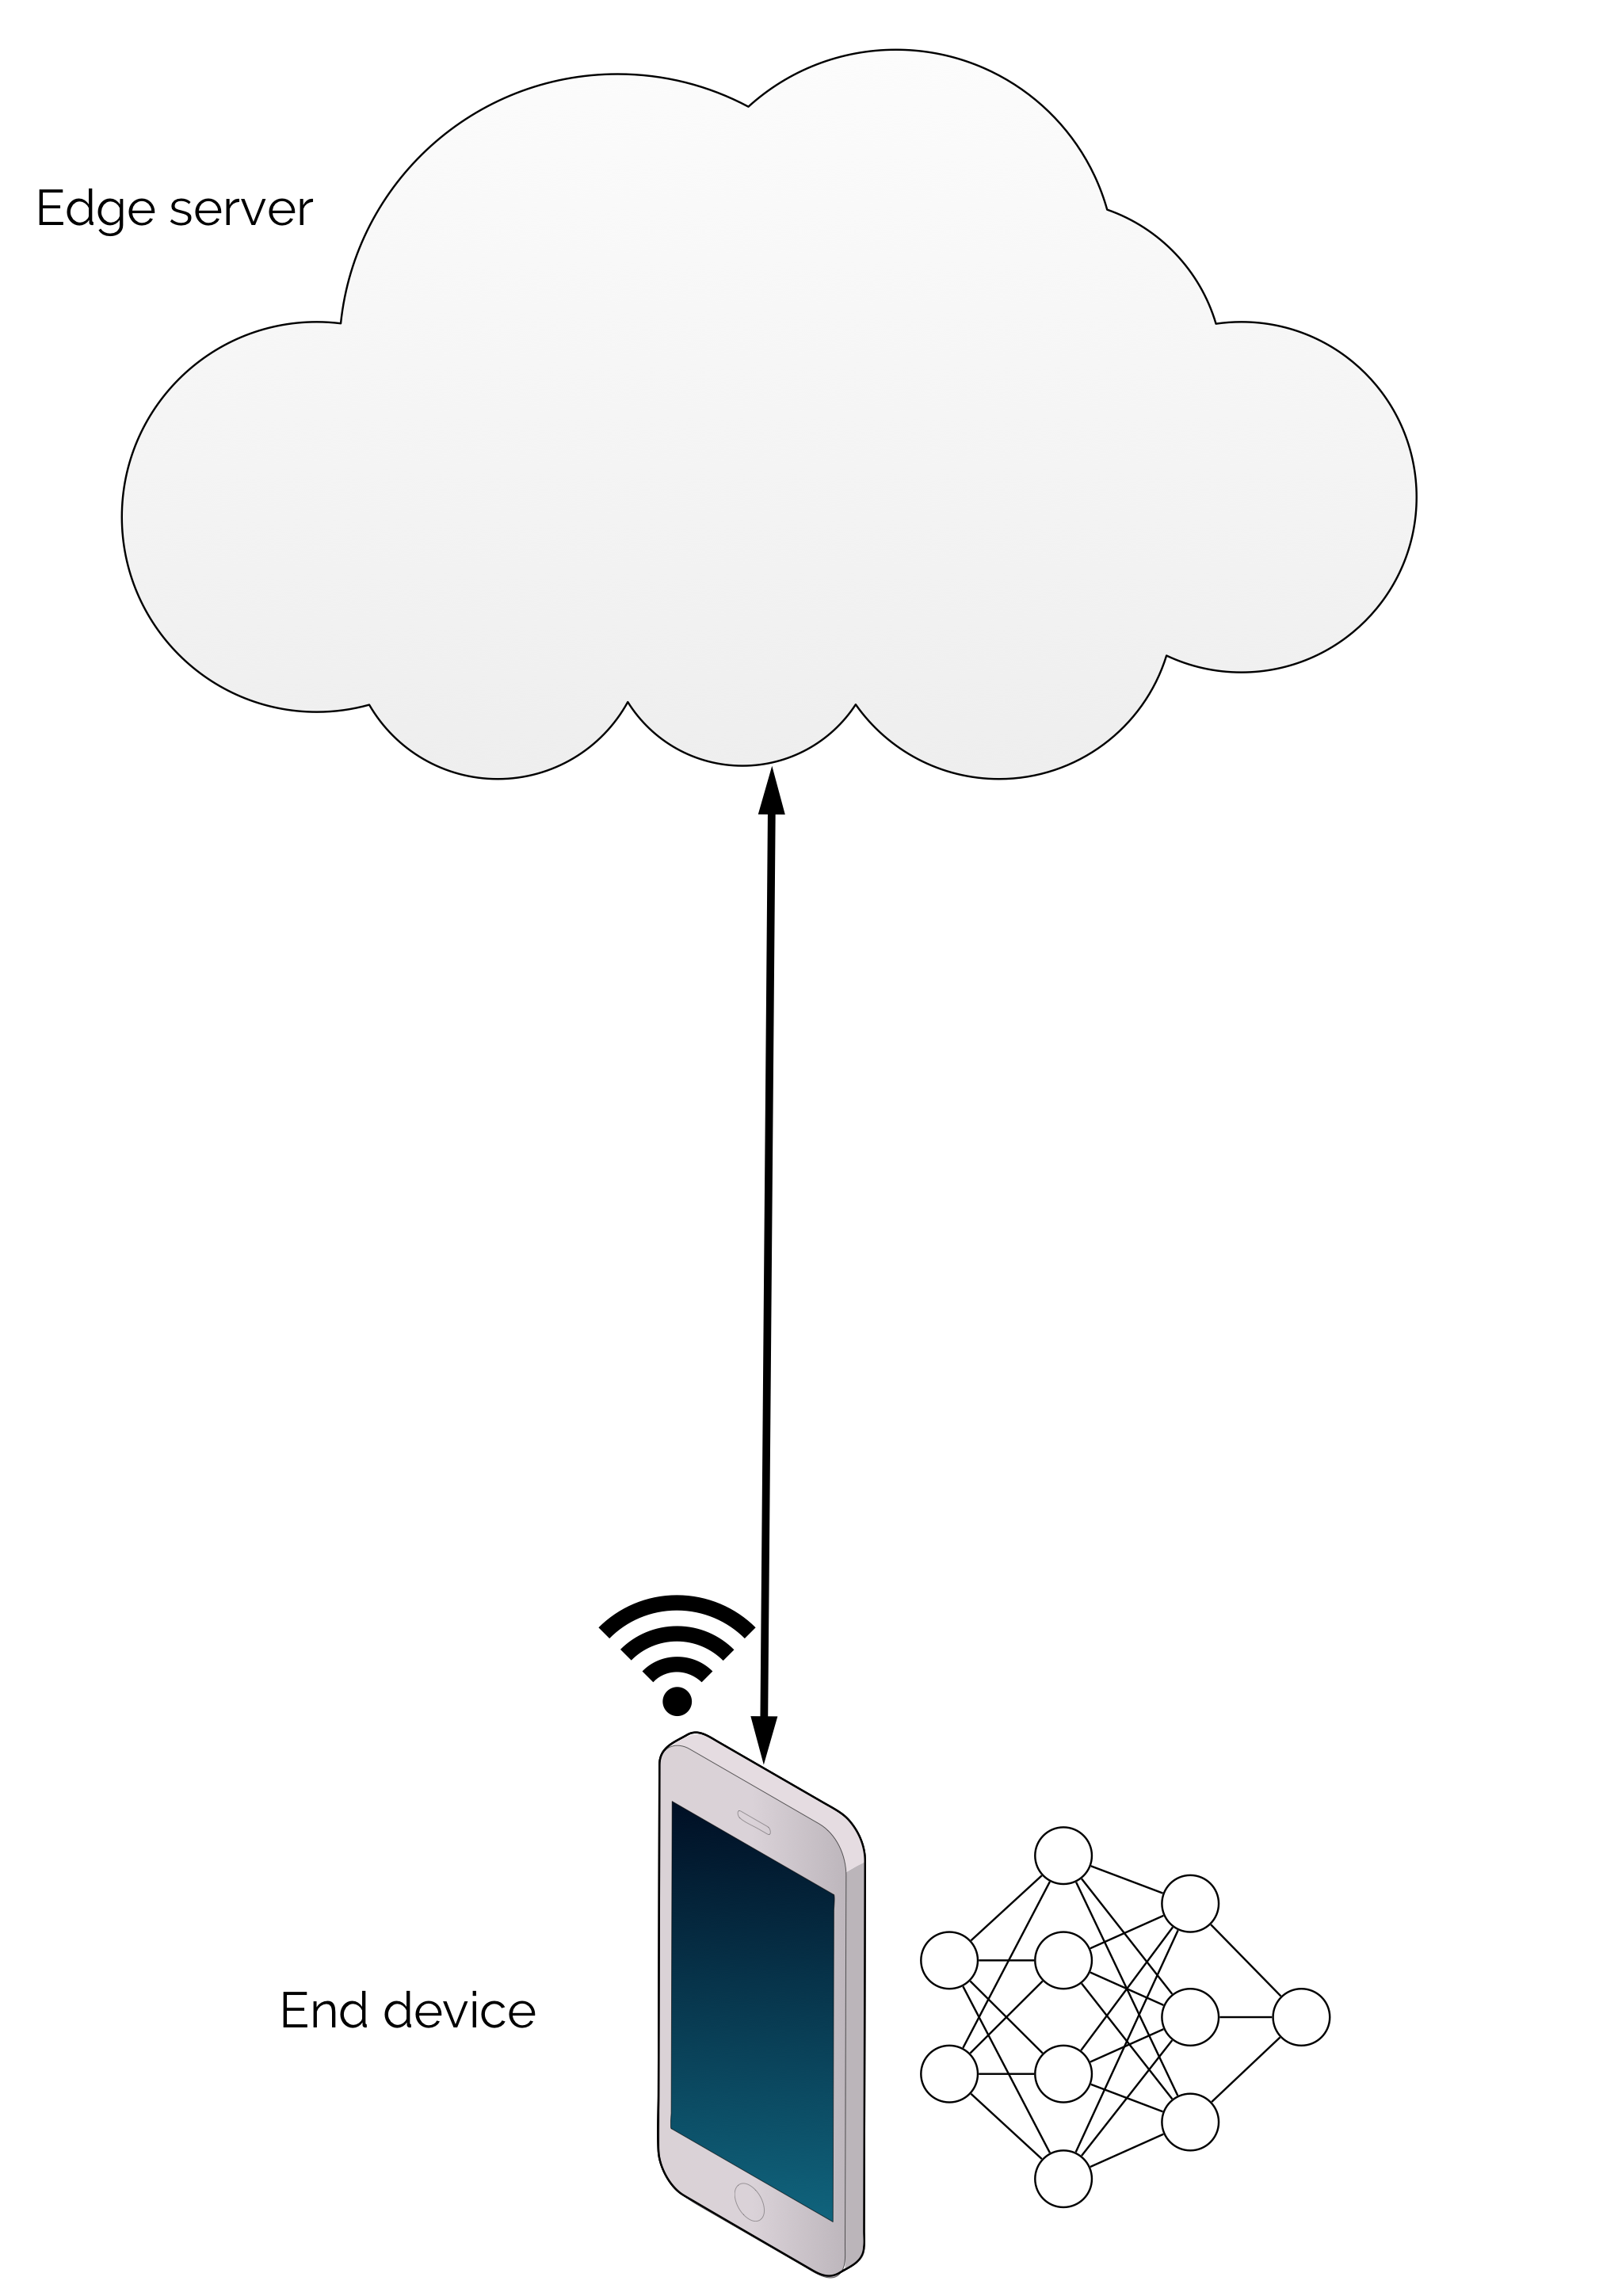
\includegraphics[width=\linewidth]{figures/models/device}}
		\end{figure}
	\end{minipage}
	
	\begin{minipage}{0.3\linewidth}
		\centering
		\begin{figure}
			\centering
			\captionsetup[subfigure]{justification=centering}
			\subfloat[Edge-based\label{fig:edge-based}]{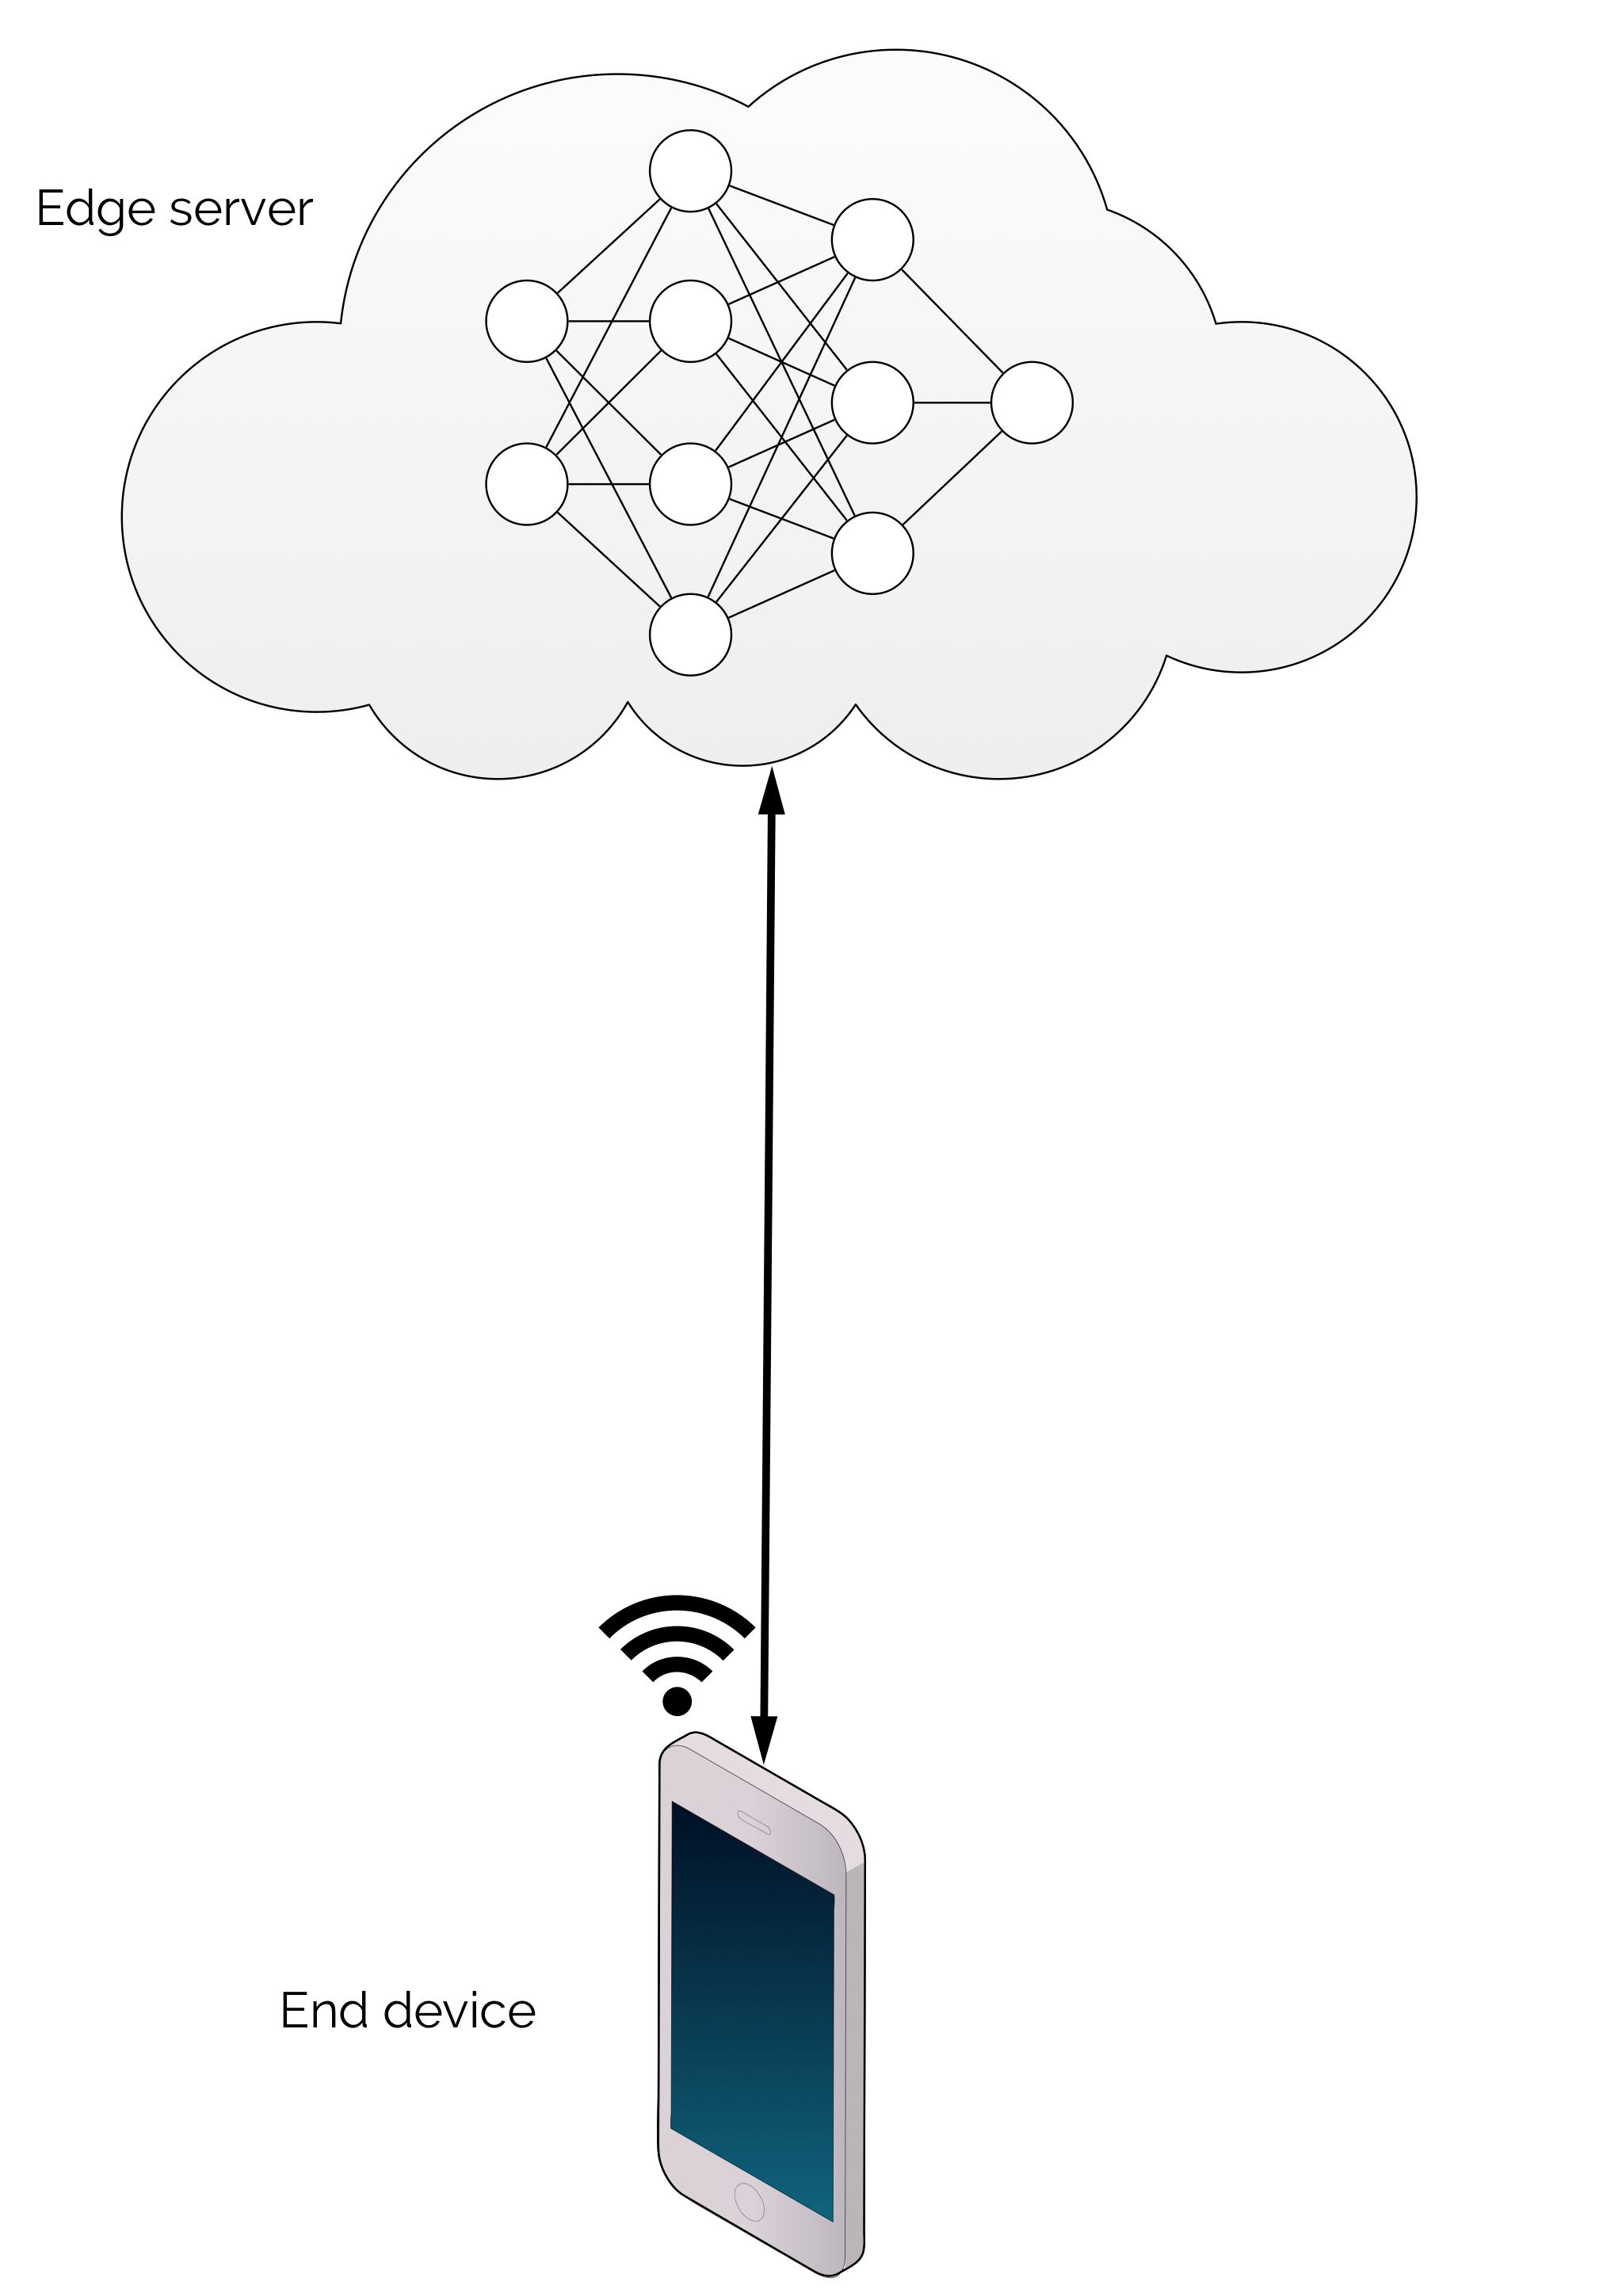
\includegraphics[width=\linewidth]{figures/models/edge}}
		\end{figure}
	\end{minipage}
	\hfill
	\begin{minipage}{0.65\linewidth}
		\textbf{\protect\subref{fig:edge-based} \textsc{Edge-based}}
		\color{caption-color} \newline
		The end device acquires input data. The input data is transferred to an edge server, which performs model inference and send the prediction results back to the end device. The performance relies on edge server computing resources and the available network bandwidth between end device and edge server. If time is the main concern remote offloading is only sensible whenever time could be saved over to local execution. Or if energy efficiency is the main concern remote offloading is only sensible if energy could be saved by communicating data instead of computing locally.
	\end{minipage}
\end{figure}

The first two modes are the conventional schemes, which resembles the current cloud-centric state, where all processing are done by one peer. The next two schemes exemplifies collaborative architectures, where processing is divided for partial execution between the peers.

\begin{figure}
	\begin{minipage}{0.65\linewidth}
		\textbf{\protect\subref{fig:edge-device-mode} \textsc{Collaborative Edge}}
		\color{caption-color} \newline
		The end device acquires input data and performs partially model inference. The intermediate data is transferred to an edge server which finalizes model inference. The performance relies on the computing resource of both the end device and the edge server and edge server workload, as well as available network bandwidth between end device and edge server. 
	\end{minipage}%
	\hfill
	\begin{minipage}{0.3\linewidth}
		\centering
		\captionsetup[subfigure]{justification=centering}
		\begin{figure}
			\centering
			\subfloat[Collaborative Edge\label{fig:edge-device-mode}]{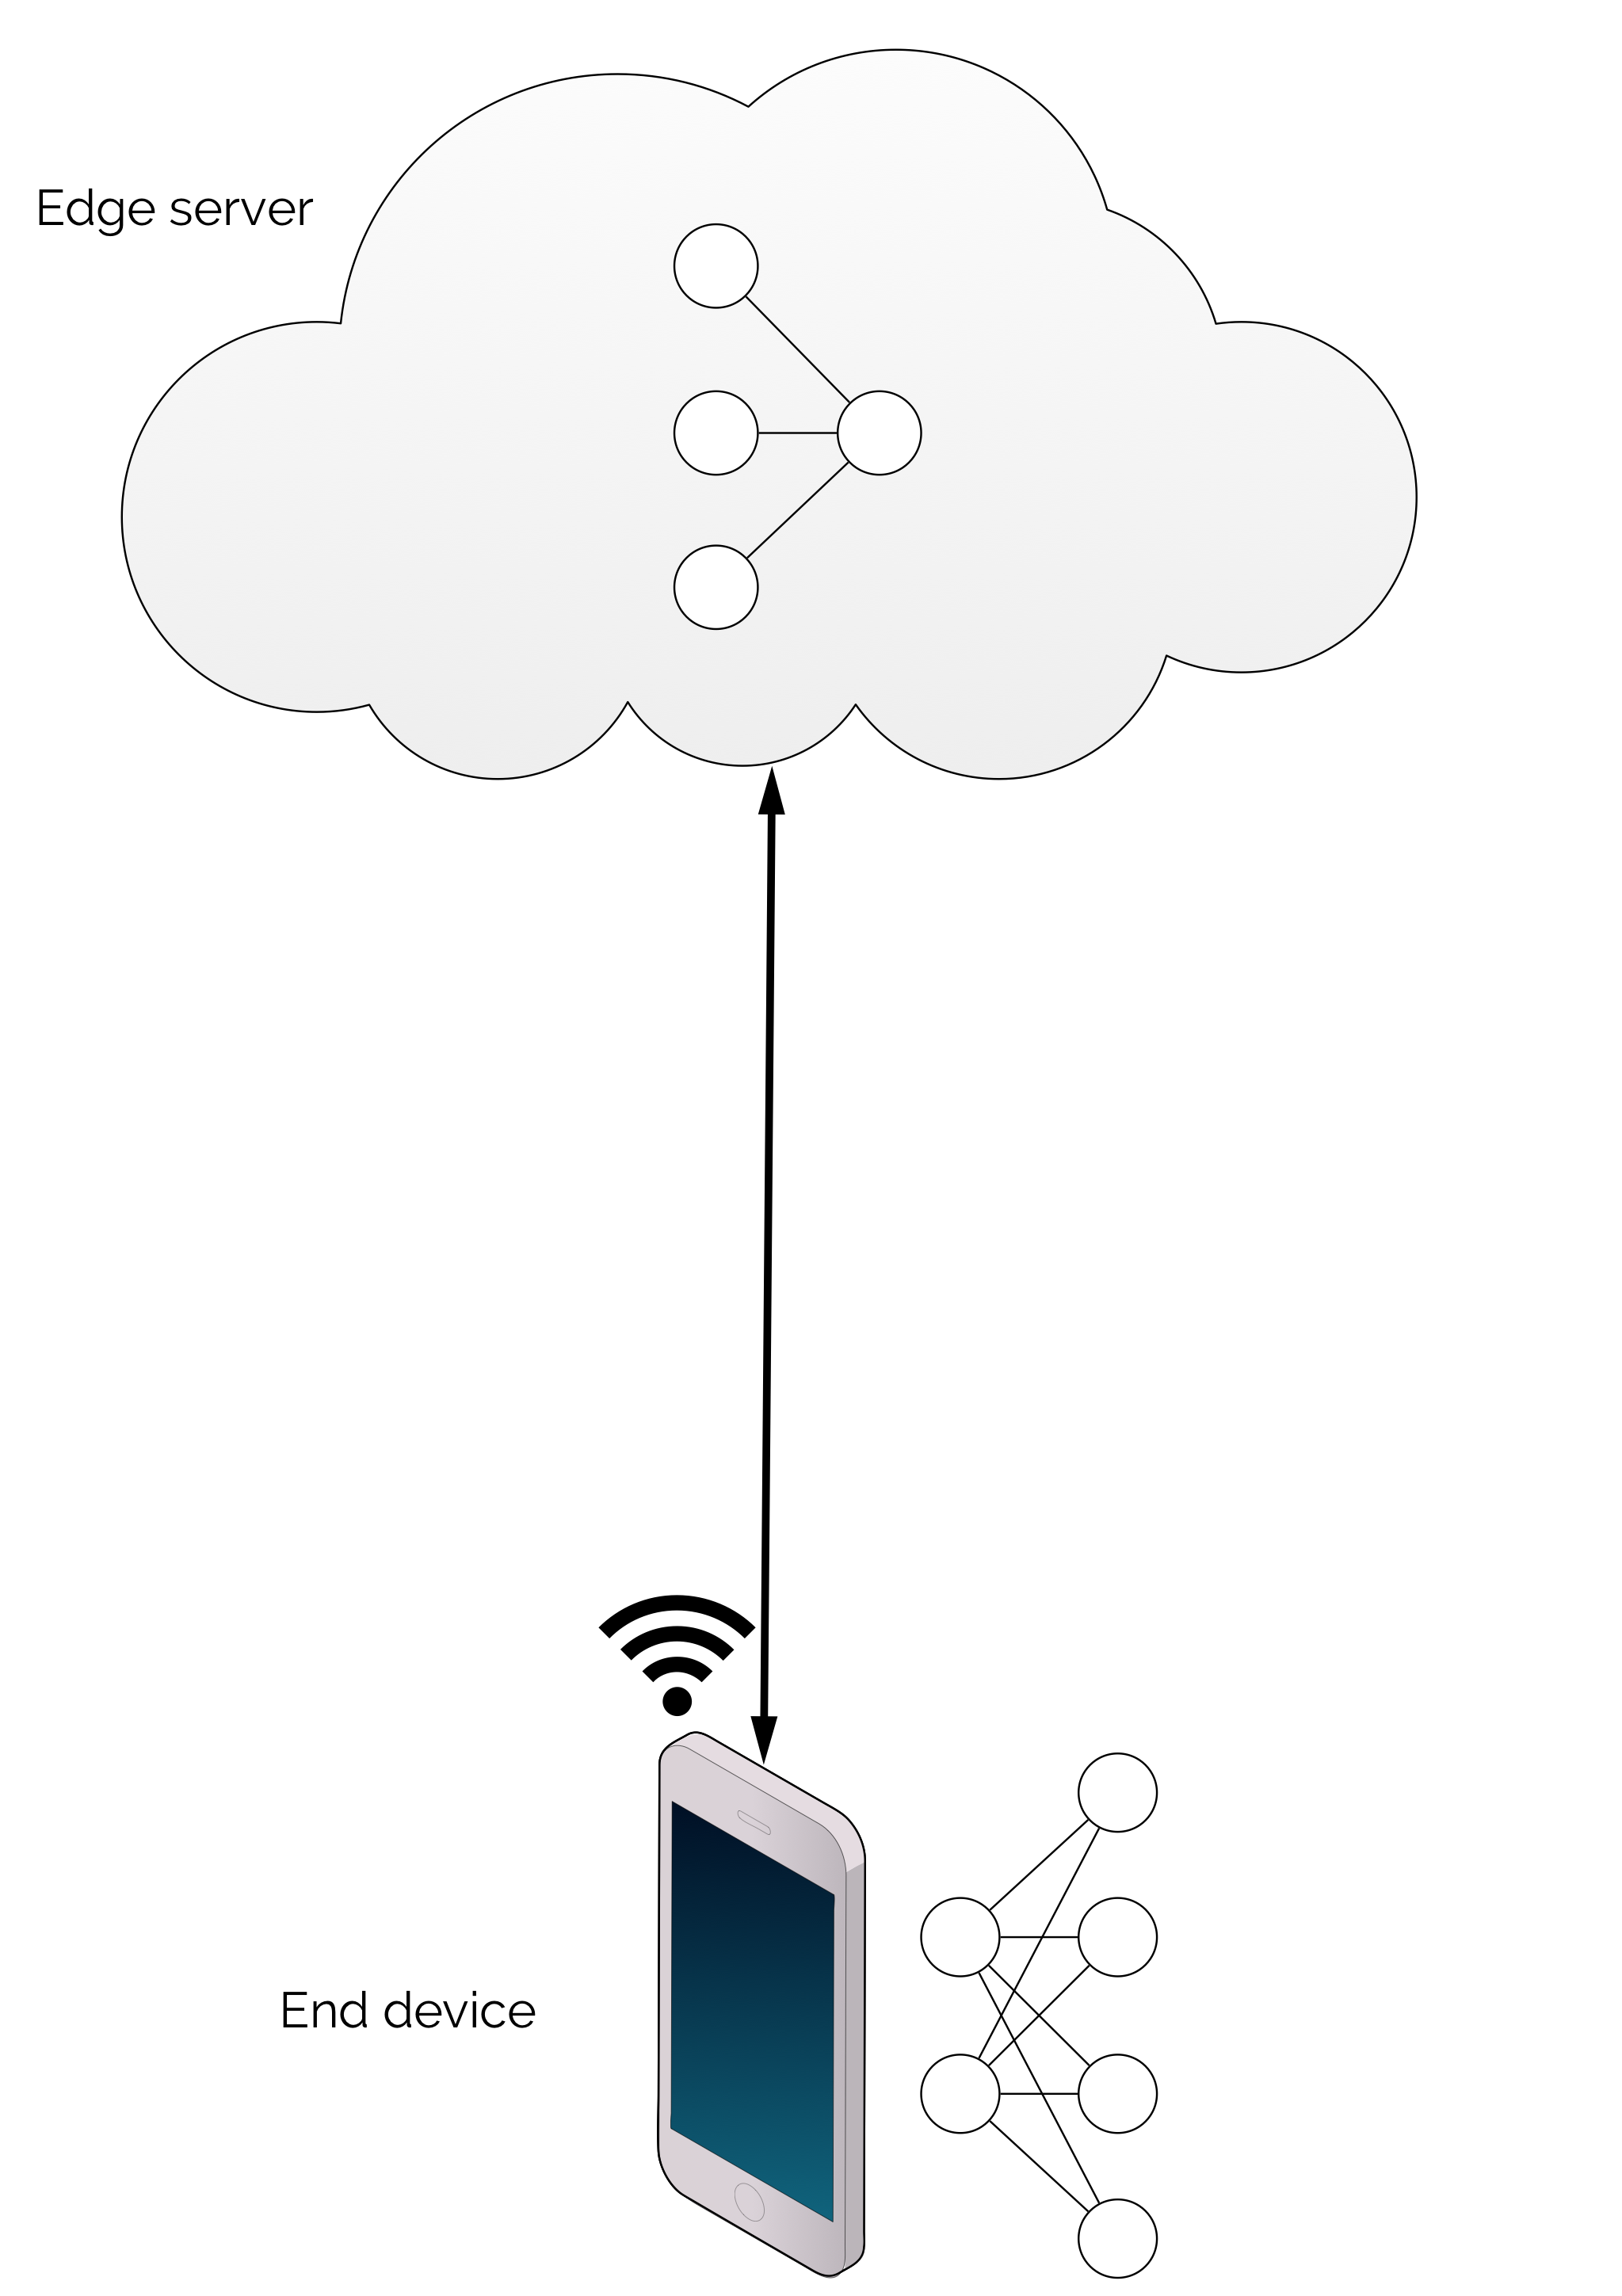
\includegraphics[width=\linewidth]{figures/models/edge_device}}
		\end{figure}
	\end{minipage}
	\begin{minipage}{0.5\linewidth}
		\centering
		\captionsetup[subfigure]{justification=centering}
		\begin{figure}
			\centering
			\subfloat[Collaborative Edge-Cloud\label{fig:edge-cloud-mode}]{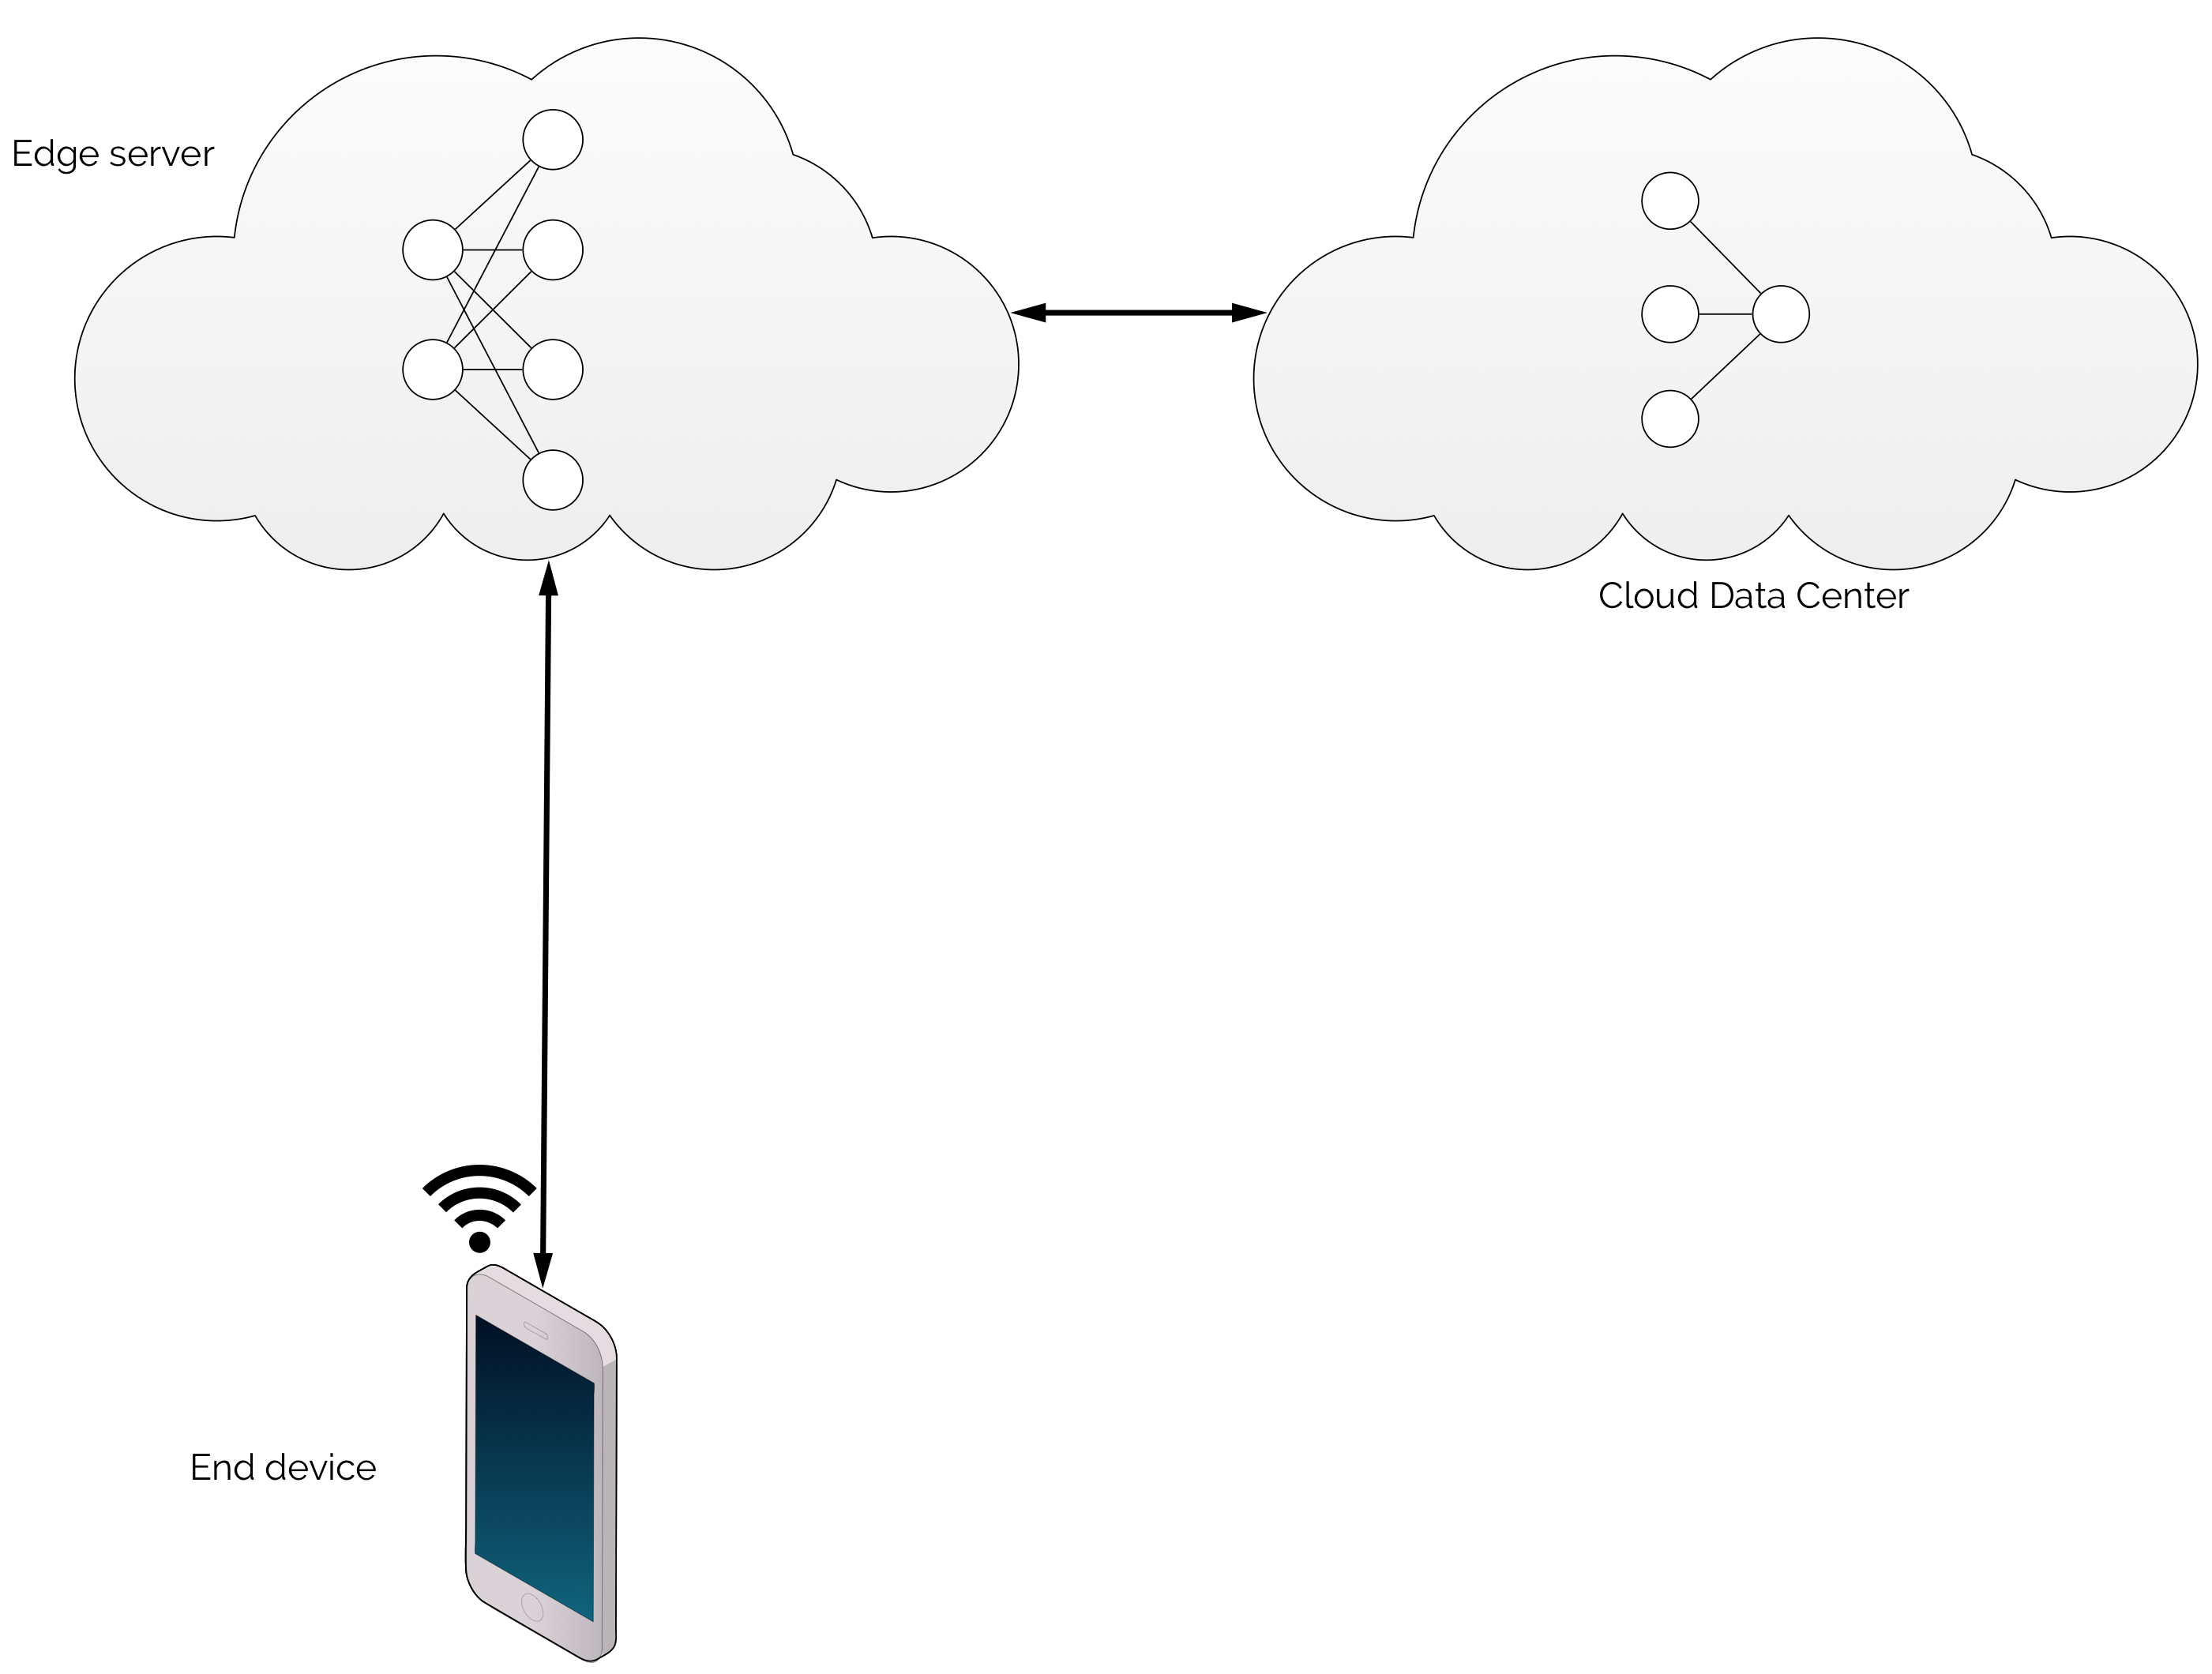
\includegraphics[width=\linewidth]{figures/models/edge_cloud}}
		\end{figure}
	\end{minipage}
	\hfill
	\begin{minipage}{0.45\linewidth}
		\textbf{\protect\subref{fig:edge-cloud-mode} \textsc{Collaborative Edge-Cloud}}
		\color{caption-color} \newline
		Resembles edge-device mode, however the model inference task is now partitioned between edge server and cloud data centers. The model is now reliant on edge server and data center computing resources, but even more so on network connection between edge and cloud.
	\end{minipage}
	\caption[Edge-centric Architectures]{Edge-centric Architectures: \protect\subref{fig:device-based} device only execution, \protect\subref{fig:edge-based} edge only execution,\protect\subref{fig:edge-device-mode} edge and device partial execution, \protect\subref{fig:edge-cloud-mode} edge and cloud partial execution}
	\label{fig:edge_arch}
\end{figure}

\begin{description}
	\item[Privacy] data generated by end devices might be confidential, hence not allowed to be processed by a data center unless confidentiality can be guaranteed. Privacy relies on how data is process within the \gls{ei} application. Offloading model input data, may be susceptible to interception, as it may be well understood by an adversary, however offloading intermediate data with no apparent meaning for humans may help improve the confidentiality of data.    
	
	\item[Memory footprint] reducing memory footprint of \gls{dnn} inference is important especially for mobile \gls{iot} devices. Mobile device do not have dedicate \gls{gpu} memory, hence \gls{dnn} application will have to compete with other applications running on both \gls{cpu} and \gls{gpu}. The resource hungry \gls{dnn} application will drain battery resources and potentially harm performance of coexisting applications. 
\end{description}
\todo{find where this should be mentioned and of course rewritten}


Over recent years interest research in reducing inference time have grown. In the next section related work will be explained.  


%Recent years breakthrough within \gls{dl} have led to a dramatic increase in the amount of \gls{ai} applications and services, such as personal assistants, recommendation systems and surveillance systems. Combined with the development of mobile computing and \gls{iot}, where billions of device are getting connected to the internet. Traditionally data for \gls{ai} applications and services are generated by the devices and transferred to large data centers for computation.    To fully unleash the power of \gls{ai} applications and services \gls{ei} or edge \gls{ai} have become an interesting research area. \gls{ei} have potential to reduce the 
  


This work is mainly concerned the accuracy-latency trade-off for inference in \gls{ei} applications and services. Thus, it will primarily address technologies regarding these performance metrics, and refer to the survey for a broader perspective on all of the performance metrics for \gls{ei} applications and services. The centralized device-based and edge-based architectures are addressed by common \gls{dl} literature. The distributed inference models for \gls{ei} is a fairly recent and promising field of research for truly enabling \gls{ai} applications and services.

According to \cite{zhou_edge_2019} there are 8 main effort to shorten inference latency, these comprises; \textit{Model Compression, Model Partition, Model Early Exit, Edge Caching, Input Filtering, Model Selection, Support Multi-Tenancy} and \textit{Application Specific Optimization} (Knowlegde Transfer Learning (student-teacher training)




%\begin{figure}
%	\centering
%	\captionsetup[subfigure]{justification=centering}
%	\subfloat[Device-based\label{fig:device-based}]{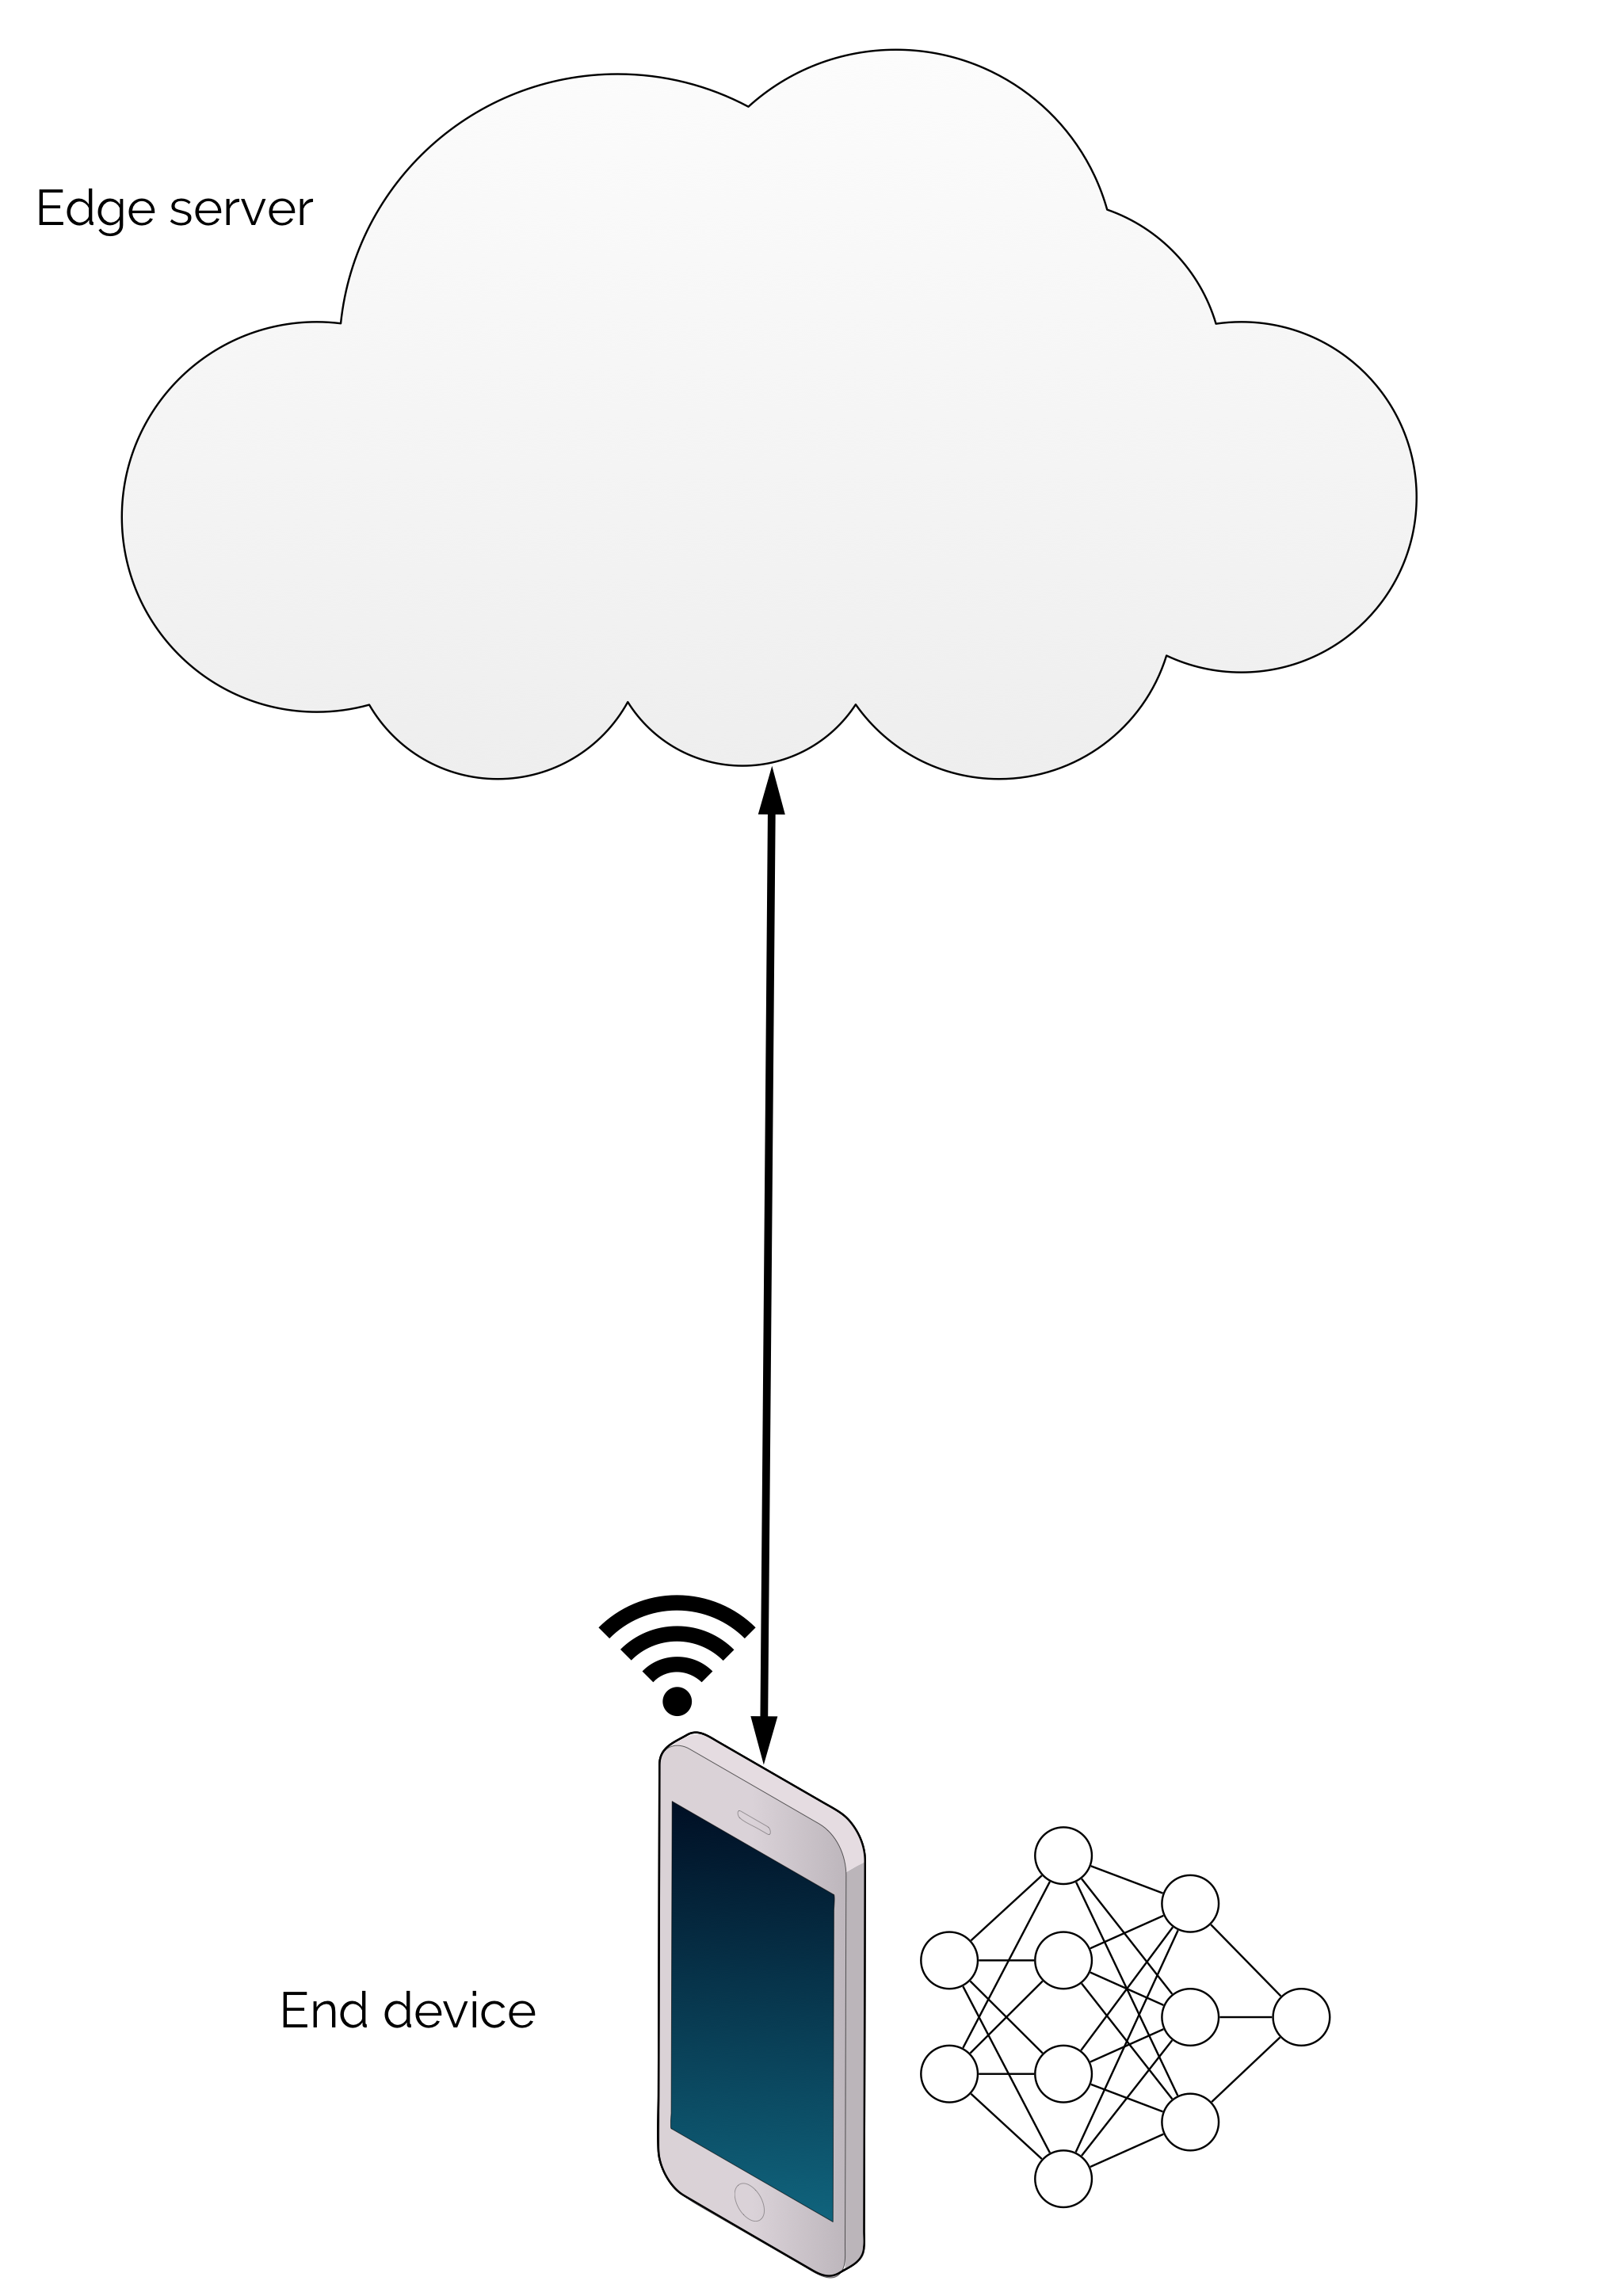
\includegraphics[width=.2\linewidth]{figures/models/device}}
%	\subfloat[Edge-based\label{fig:edge-based}]{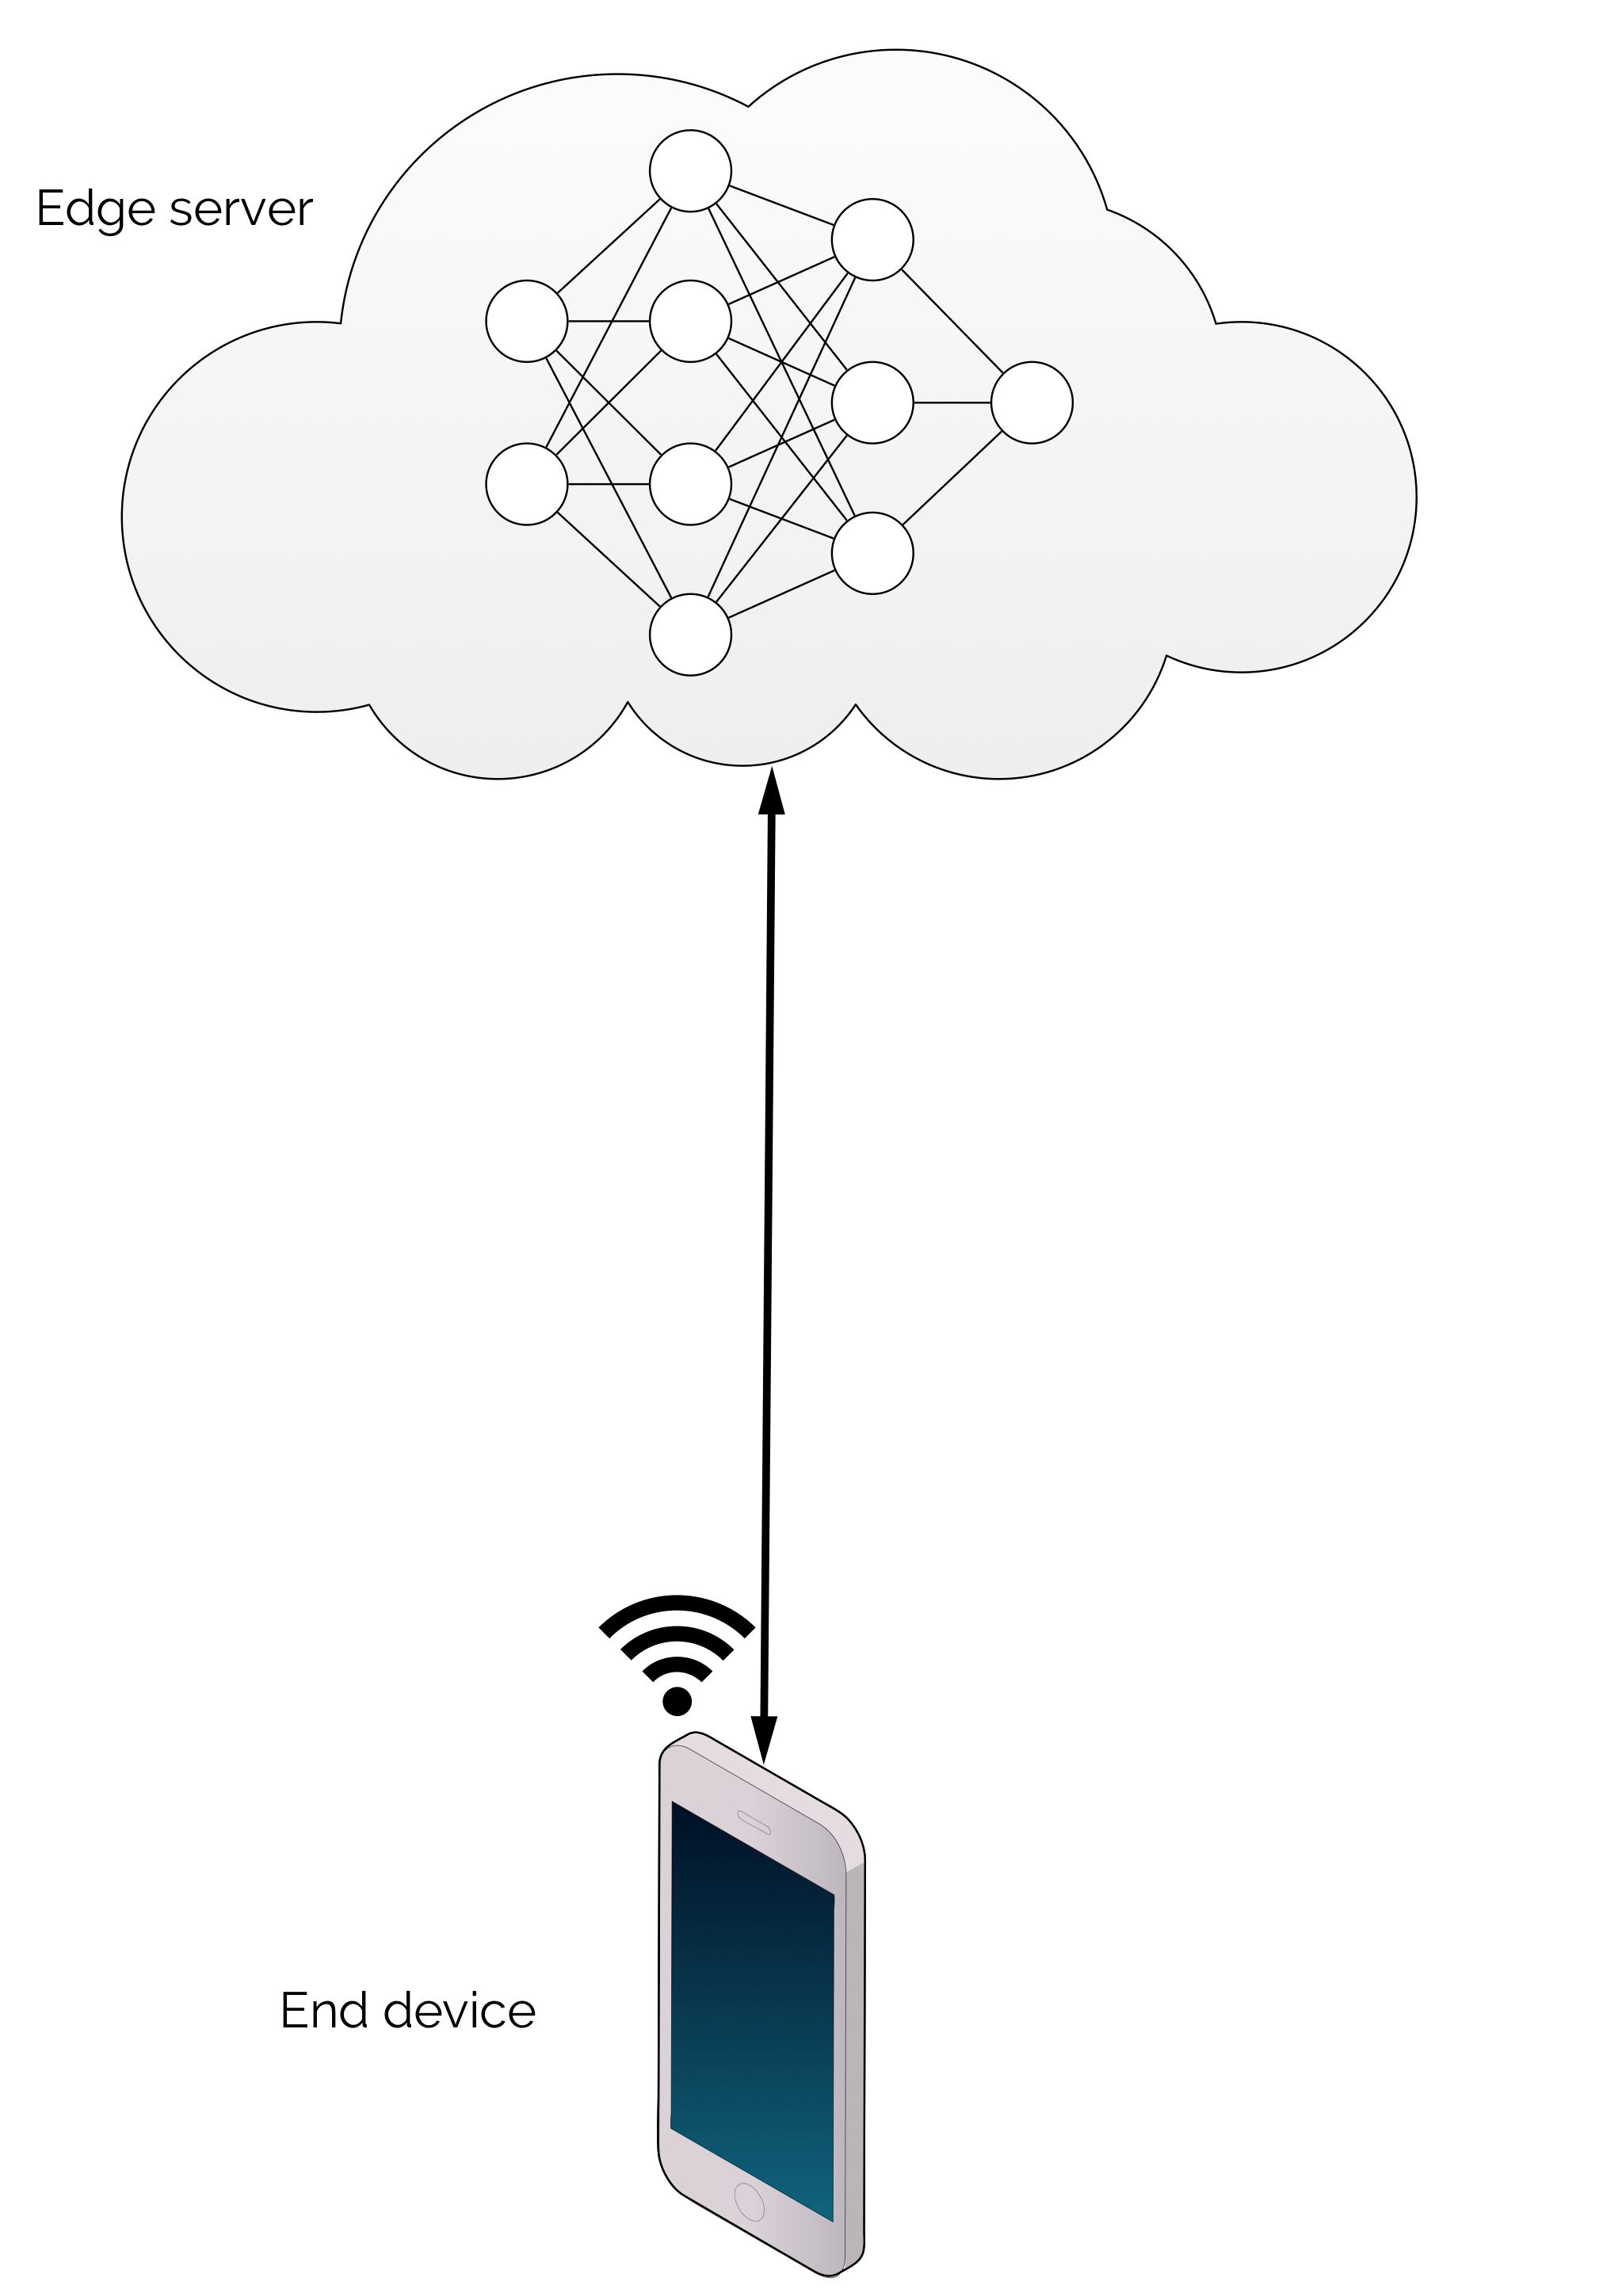
\includegraphics[width=.2\linewidth]{figures/models/edge}}
%	\subfloat[Edge-Device mode\label{fig:edge-device-mode}]{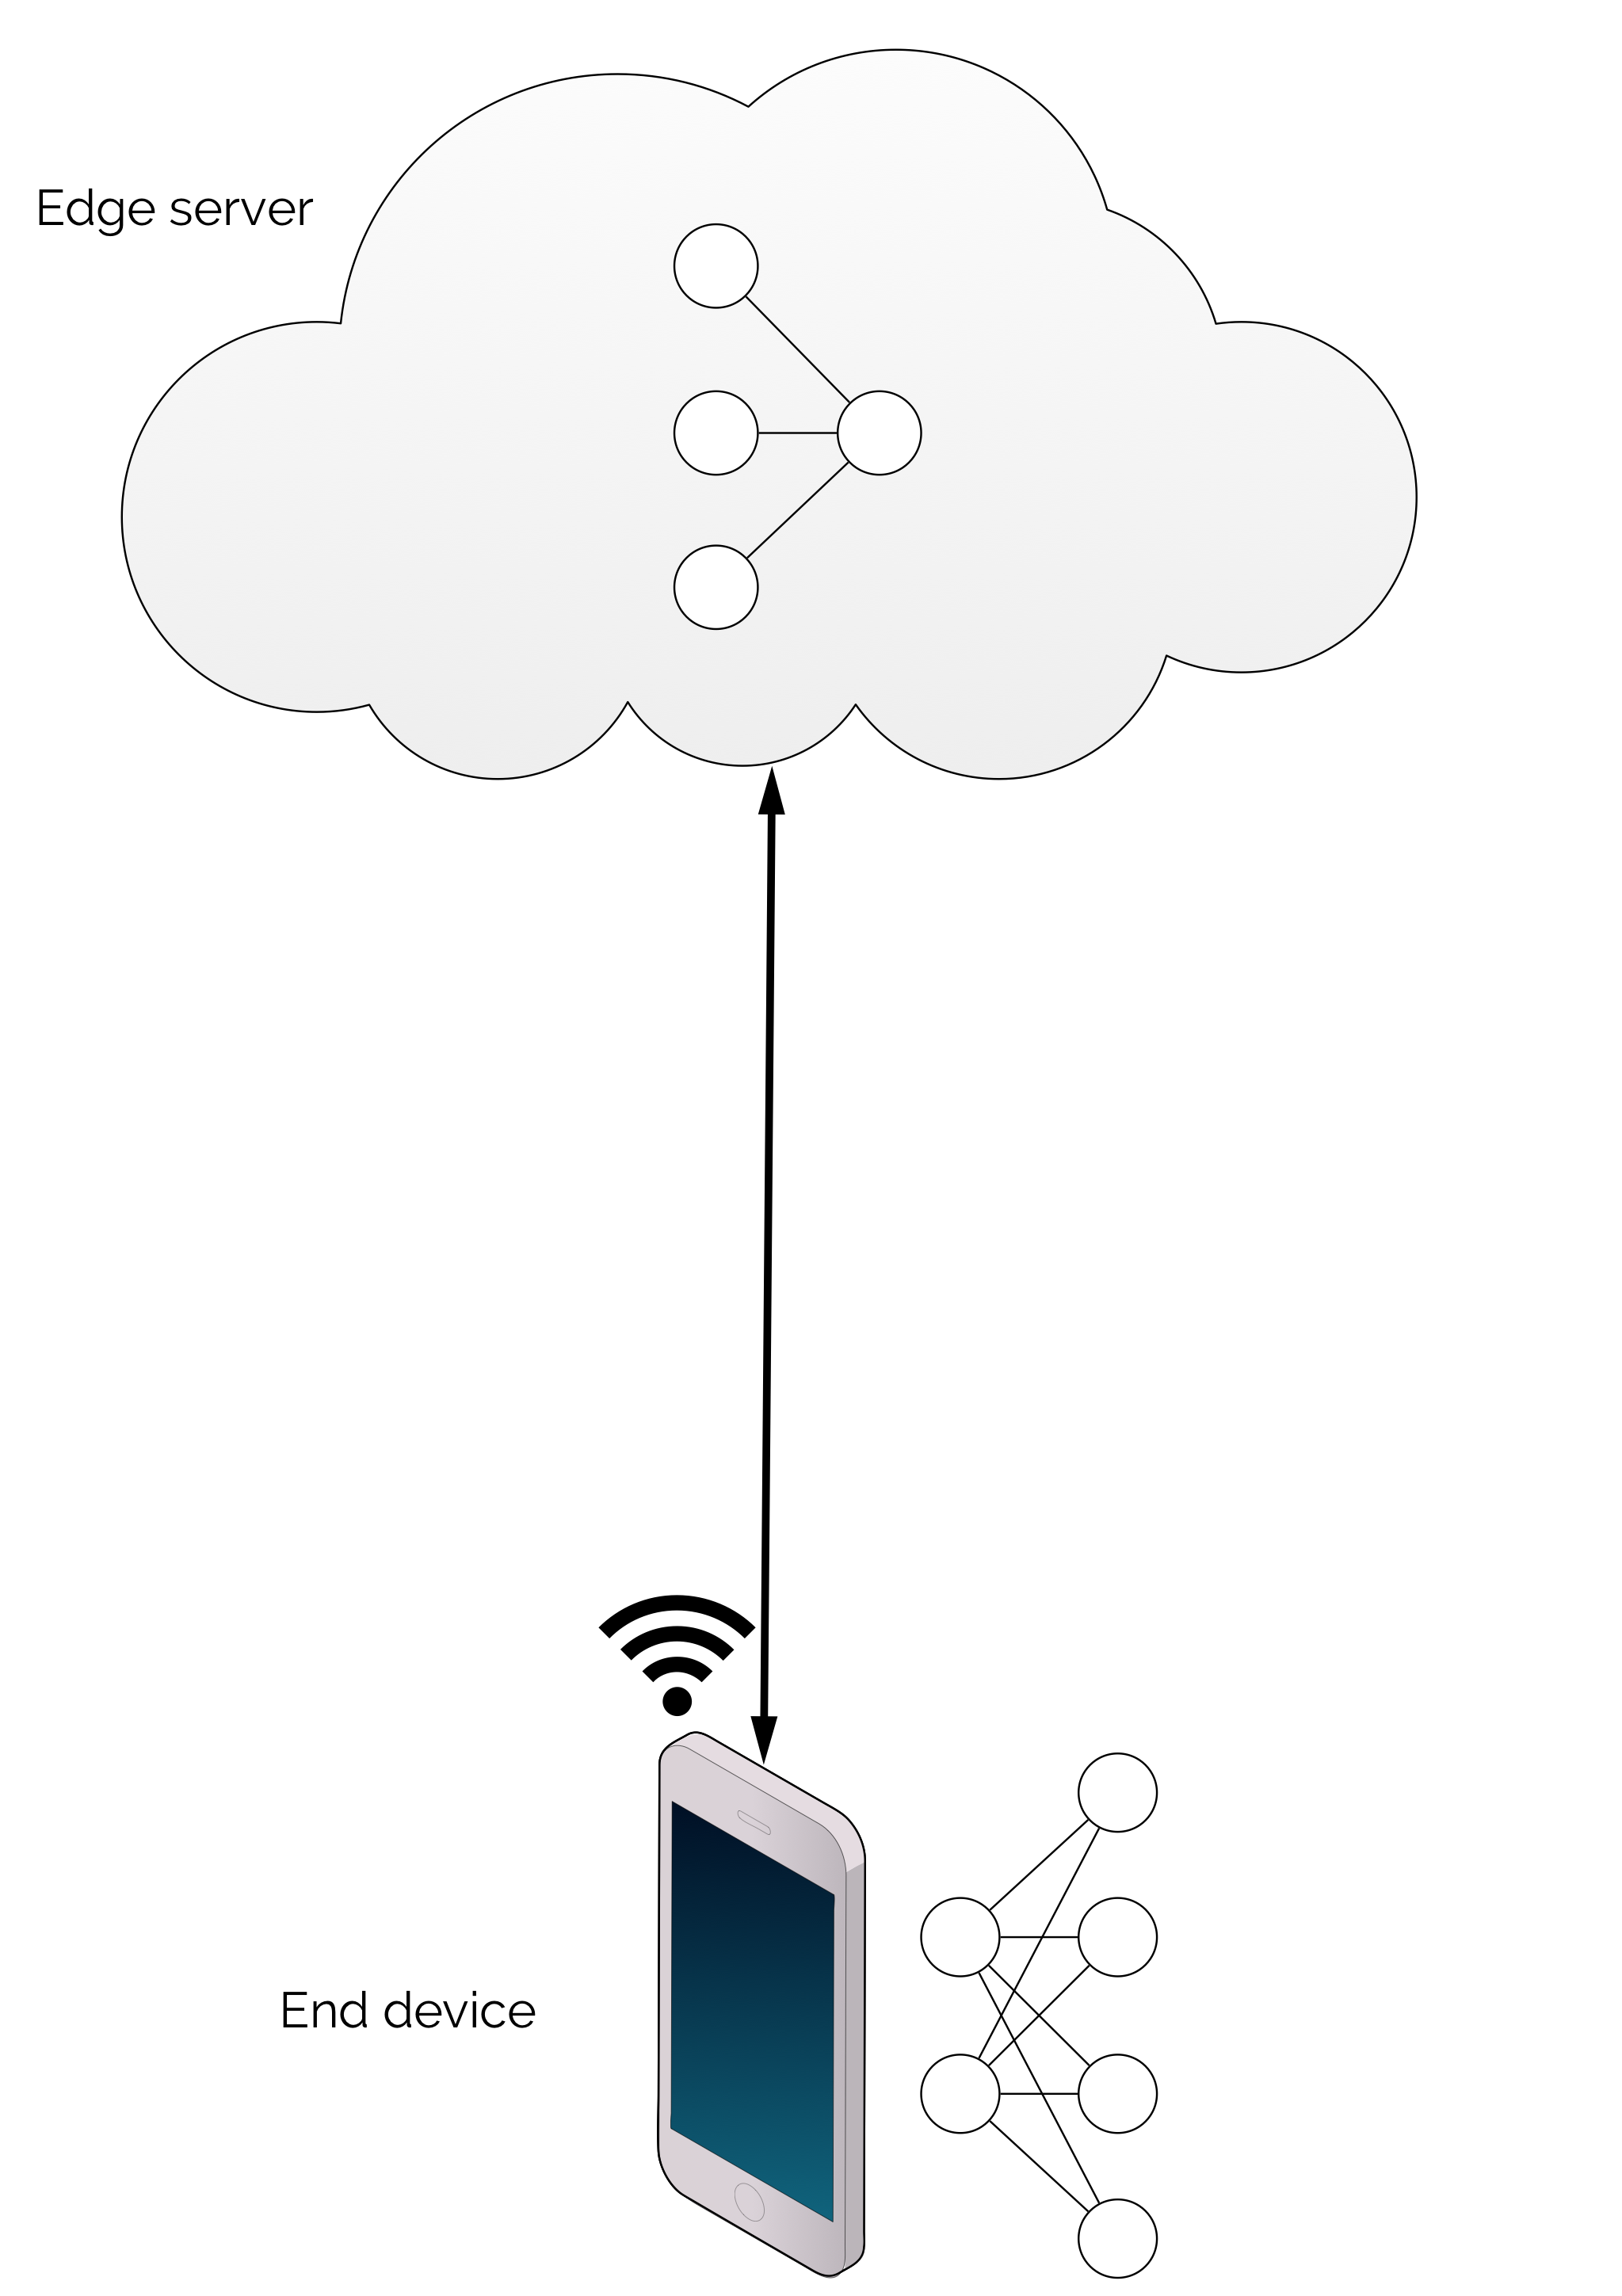
\includegraphics[width=.2\linewidth]{figures/models/edge_device}}
%	\subfloat[Edge-Cloud mode\label{fig:edge-cloud-mode}]{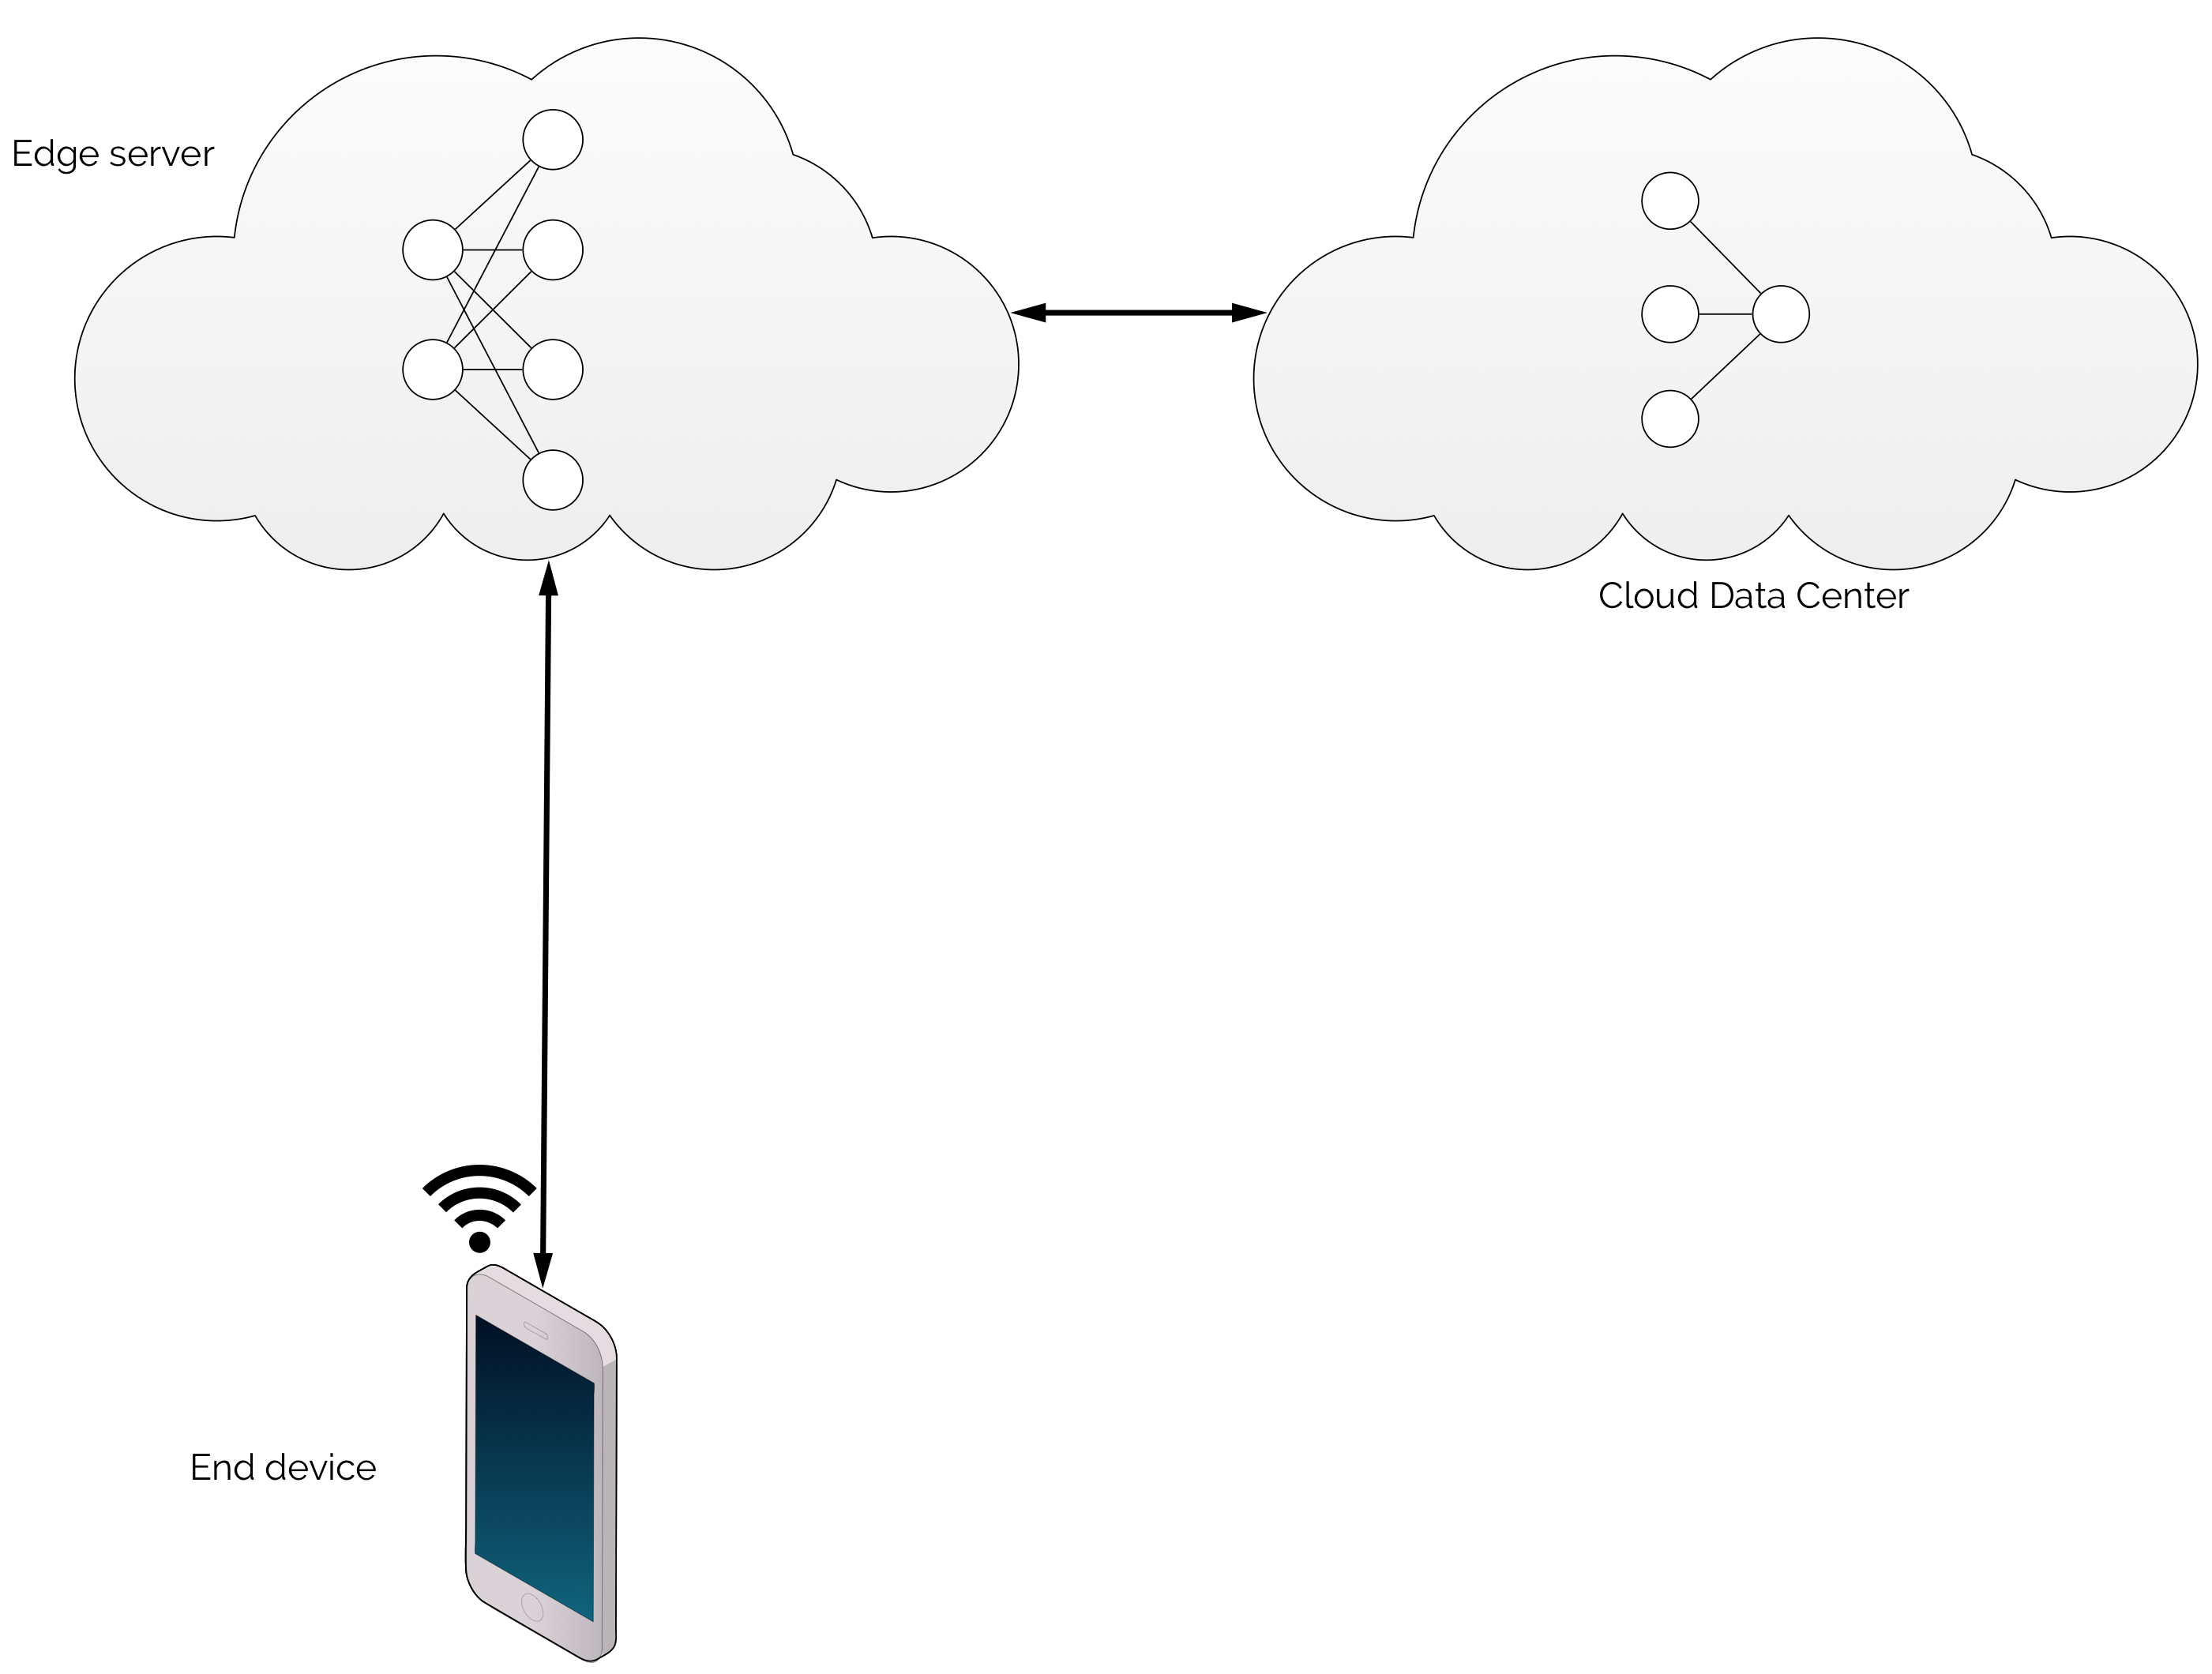
\includegraphics[width=.37\linewidth]{figures/models/edge_cloud}}
%	\caption[Edge-centric architectures]{Edge Architectures: \protect\subref{fig:device-based} device only execution, \protect\subref{fig:edge-based} edge only execution,\protect\subref{fig:edge-device-mode} edge and device partially execution, \protect\subref{fig:edge-cloud-mode} edge and cloud partially execution. }
%\end{figure}
%
%\begin{description}
%	\item[Device-based Mode]
%	 end device obtain model from edge server. The end-device then acquires input data and performs model inference. Since all computation is done on the end device, performance is solely reliant on the end device's computing resources. 
%	
%	\item[Edge-based Mode] end device acquires input data. The input data is transferred to an edge server, which performs model inference and send the prediction results to the end device. The performance relies on edge server computing resources and network bandwidth.
%	\item[Edge-Device Mode] end device acquires input data and performs partially model inference. The intermediate data is transferred to an edge server which finalizes model inference. The performance relies on end device's and edge server computing resource, network bandwidth and edge server workload. 
%	\item[Edge-Cloud Mode] resemble edge-device mode, however the model inference task is now partitioned between edge server and cloud data centers. The model is now reliant on edge server and data center computing resources, but even more reliant on \gls{wan} transmission rate between edge and cloud. 
%\end{description}


\section{State of the Art}

\todo{introduction}

\subsection{Model Architectures}

To improve inference latency on a model-basis, efforts have been made in designing \gls{dnn}s, that reduces the amount of parameter and to more efficiently run on mobile device. Commonly for \gls{mobilenet}s \cite{howard_mobilenets:_2017,sandler_mobilenetv2:_2018}, \gls{shufflenet}s \cite{zhang_shufflenet:_2017, ma_shufflenet_2018} and \gls{squeezenet}s \cite{iandola_squeezenet:_2016} are all aiming to efficiently reducing the number of parameters, without compromising model accuracy by designing novel \gls{dnn} architectures.

Use MobileNet's inverted Linear bottlenek as example and use source that describes the parameter efficiency og this model. 

\citeauthor{sandler_mobilenetv2:_2018} designed \textsl{MobileNetV2} is a neural network architecture specifically for mobile devices. The main novelty is \textit{"inverted residual with linear bottlenecks"} a neural network layer module. \todo{ELABORATE}

Furthermore it uses another type of convolutional layer \textit{depth-wise separable convolutions}, both of which seeking to decrease the number of parameters. \todo{ELABORATE}

Other efforts have been made to reduce the number of parameters, thus the inference time in state-of-the-art model compression. 

\subsection{Model Compression}

A the name impliese model compression is all about finding a more compact or compressed way to represent the model. Weight pruning is one of such methods. Weight pruning is the removal of redundant weights, which have shown significant speed-ups using with a small loss in accuracy \cite{zhou_edge_2019}. The impact of compression is application dependent and can be applied to any pretrained \gls{dnn} and in combination with other techniques \cite{cheng_survey_2017}.

Another compression technique is quantization. A more compact representation of a floating point is used to reduce the amount of bits needed for each weight of the model \cite{cheng_survey_2017}. The extreme case is binarization, where weights and activations are learned as a binary representations. In BinaryConnect \cite{courbariaux_binaryconnect:_2015} and \gls{bnn} \cite{courbariaux_binarized_2016} most arithmetic operations are replaced with bit-wise operations, thus greatly improving the power-efficiency and inference latency, however using binary weights in extremely deep network have shown significant degradation in accuracy \cite{cheng_survey_2017}.

In \cite{hinton_distilling_2015} \gls{kd} has been proposed. \gls{kd} is a framework to train \gls{dnn} in a student-teacher paradigm. The student network are penalized using the output of an ensemble of teacher networks. \gls{kd} can be viewed as a compression of an ensemble of teacher network into a student network \cite{cheng_survey_2017}. 
In \cite{romero_fitnets:_2014} \gls{fitnet} have been proposed as a method to train thinner and shallower student networks using a deeper teacher network. FitNet learns the student network to mimick the teacher network, however this approach require the softmax loss function, which limits iys usage \cite{cheng_survey_2017}.  

Other approaches specifically related to edge computing aiming to reduce inference latency, is model partitioning between end device and edge server. 

\subsection{Model Partitioning}

Model partitioning is an approach to reduce inference latency on an architectural level. Instead of solely executing a \gls{dnn} in the cloud, edge or on device, the computing resources collaborates to boost inference time. 

Splitting a model is an inherent nature of sequential \gls{dnn}s, that at any layer can be stopped. The intermediate output are transferred over the network and continued at the next layer on an edge server, as shown in figure \ref{fig:offlaoding}.

\begin{figure}
	\centering
	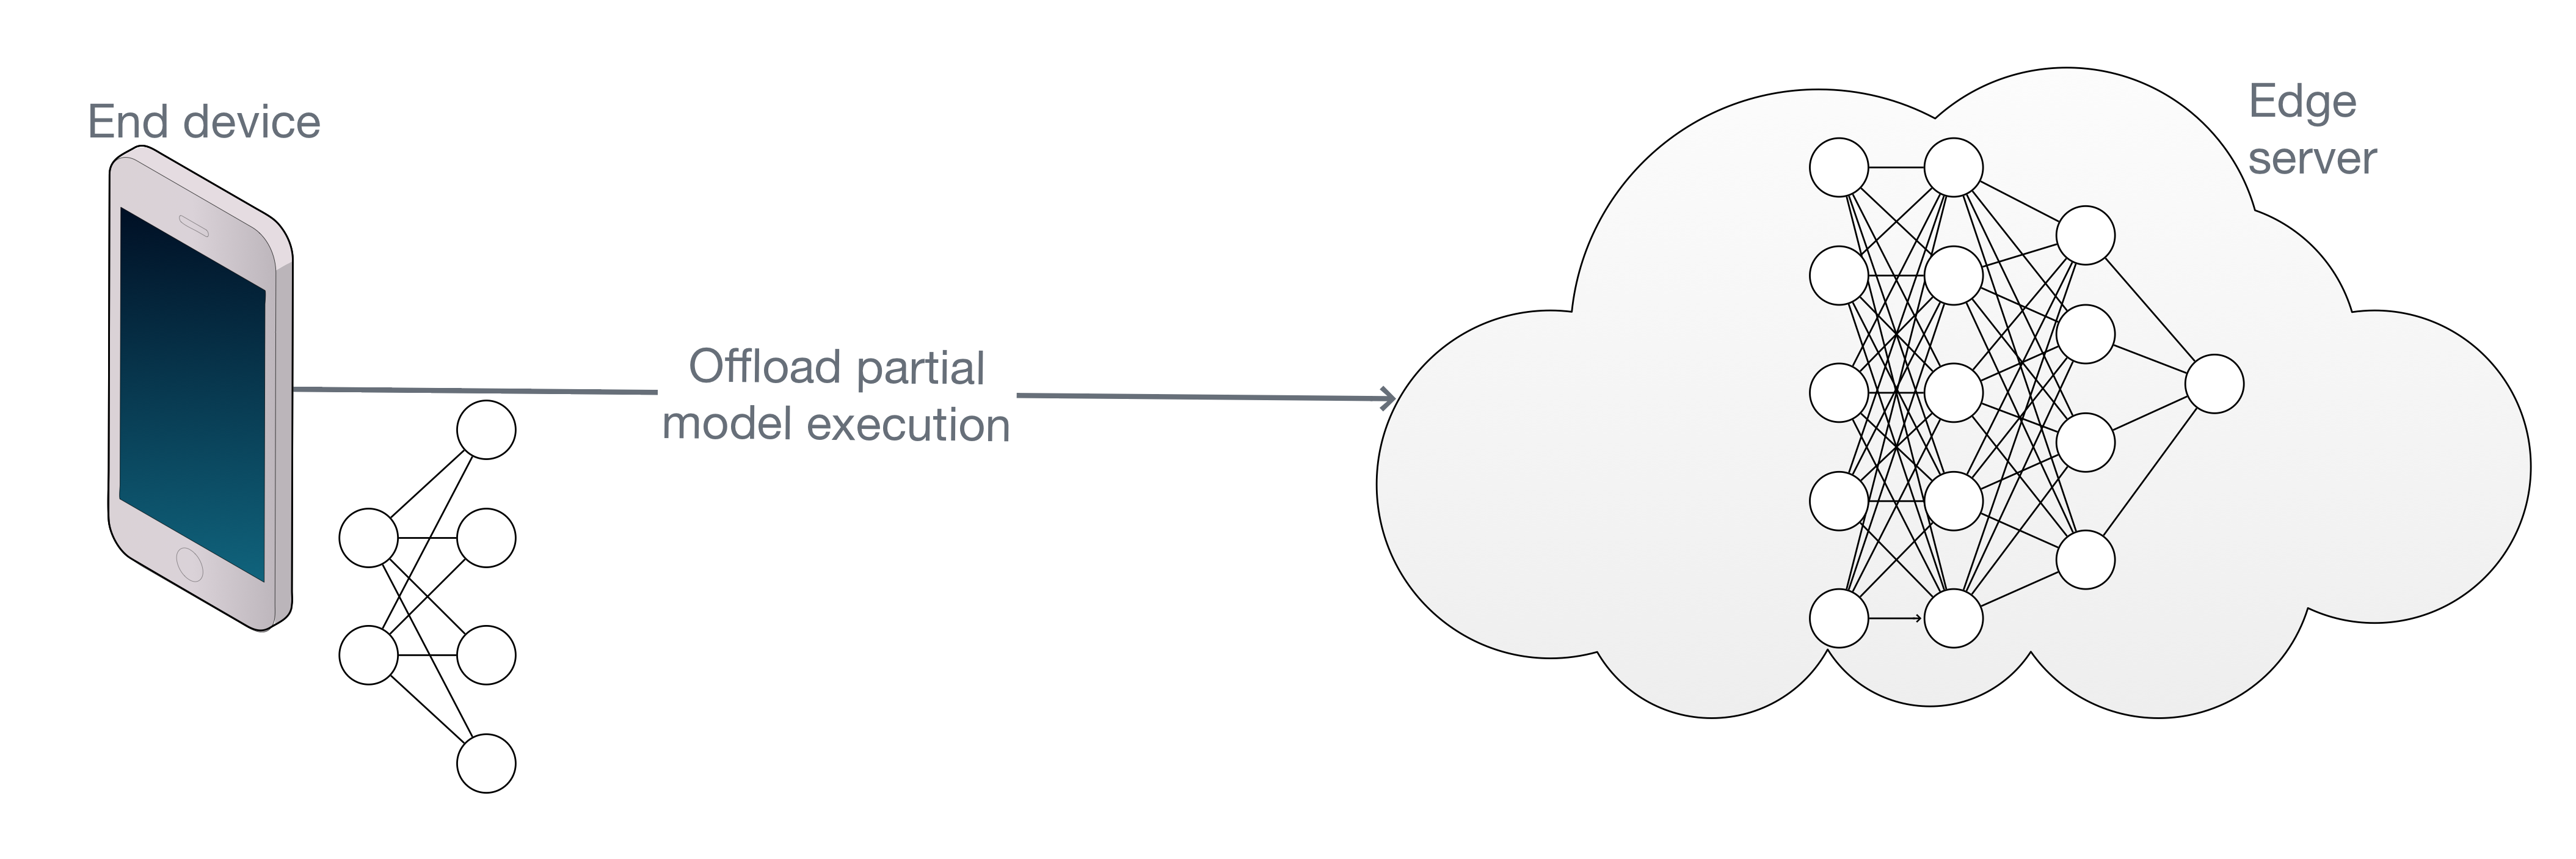
\includegraphics[width=\linewidth]{figures/models/partitioning}
	\caption[Model partitioning]{Edge-Device model partitioning run part of the model on-device and offload the rest to edge processing. Network partitioning utilize the assumption, that at some later point in the \gls{dnn} a smaller representation of the data is found, illustrated by the gradually decreasing model layers, to reduce the communication bottleneck. }
	\label{fig:offlaoding}
\end{figure}

Neurosurgeon \cite{kang_neurosurgeon:_2017} is a lightweight partitioning scheduler, that uses knowledge of the individual layers of the \gls{dnn} to effectively reduce inference latency. Communication latency is the bottleneck in an offloading application, hence a smaller representation of the input data is needed, however the layers producing a smaller output than the original input typically lies deep within the network. Neurosurgeon construct regression models for layer execution time and  output data size of the layers of a \gls{dnn}, to decide the best partition of the \gls{dnn} based on networking condition. The work is based on \gls{mcc}\todo{or cloud intelligence? which to use?} and shows, that the conventional cloud-only approach is insufficient due to different networking technologies and mobile device is becoming \gls{gpu} enabled. 
% Evidently moving computation to the edge reduces the communication latency. 

Another effort to reduce communication overhead of network splitting is adding feature compression of intermediate features before offloading to cloud or edge \cite{choi_deep_2018}. The paper shows, that lossless compression have no impact on accuracy, however bit saving is rather limited. Lossy compression, on the other hand, results in 70\% bit savings, however also affects the accuracy of the model and require compression-aware training to compensate. The follow up paper \cite{choi_near-lossless_2018} propose a novel compression techniques designed for deep features i.e. the output of a intermediate \gls{dnn} layer and achieve significant better bit saving, than conventional image compression algorithms such as JPEG. Alternatively methods such as \gls{bottlenet} uses layers of a \gls{dnn} to create a low dimensional representation of the output features, that can be restored back to original dimensionality. 

\begin{figure}
	\centering
	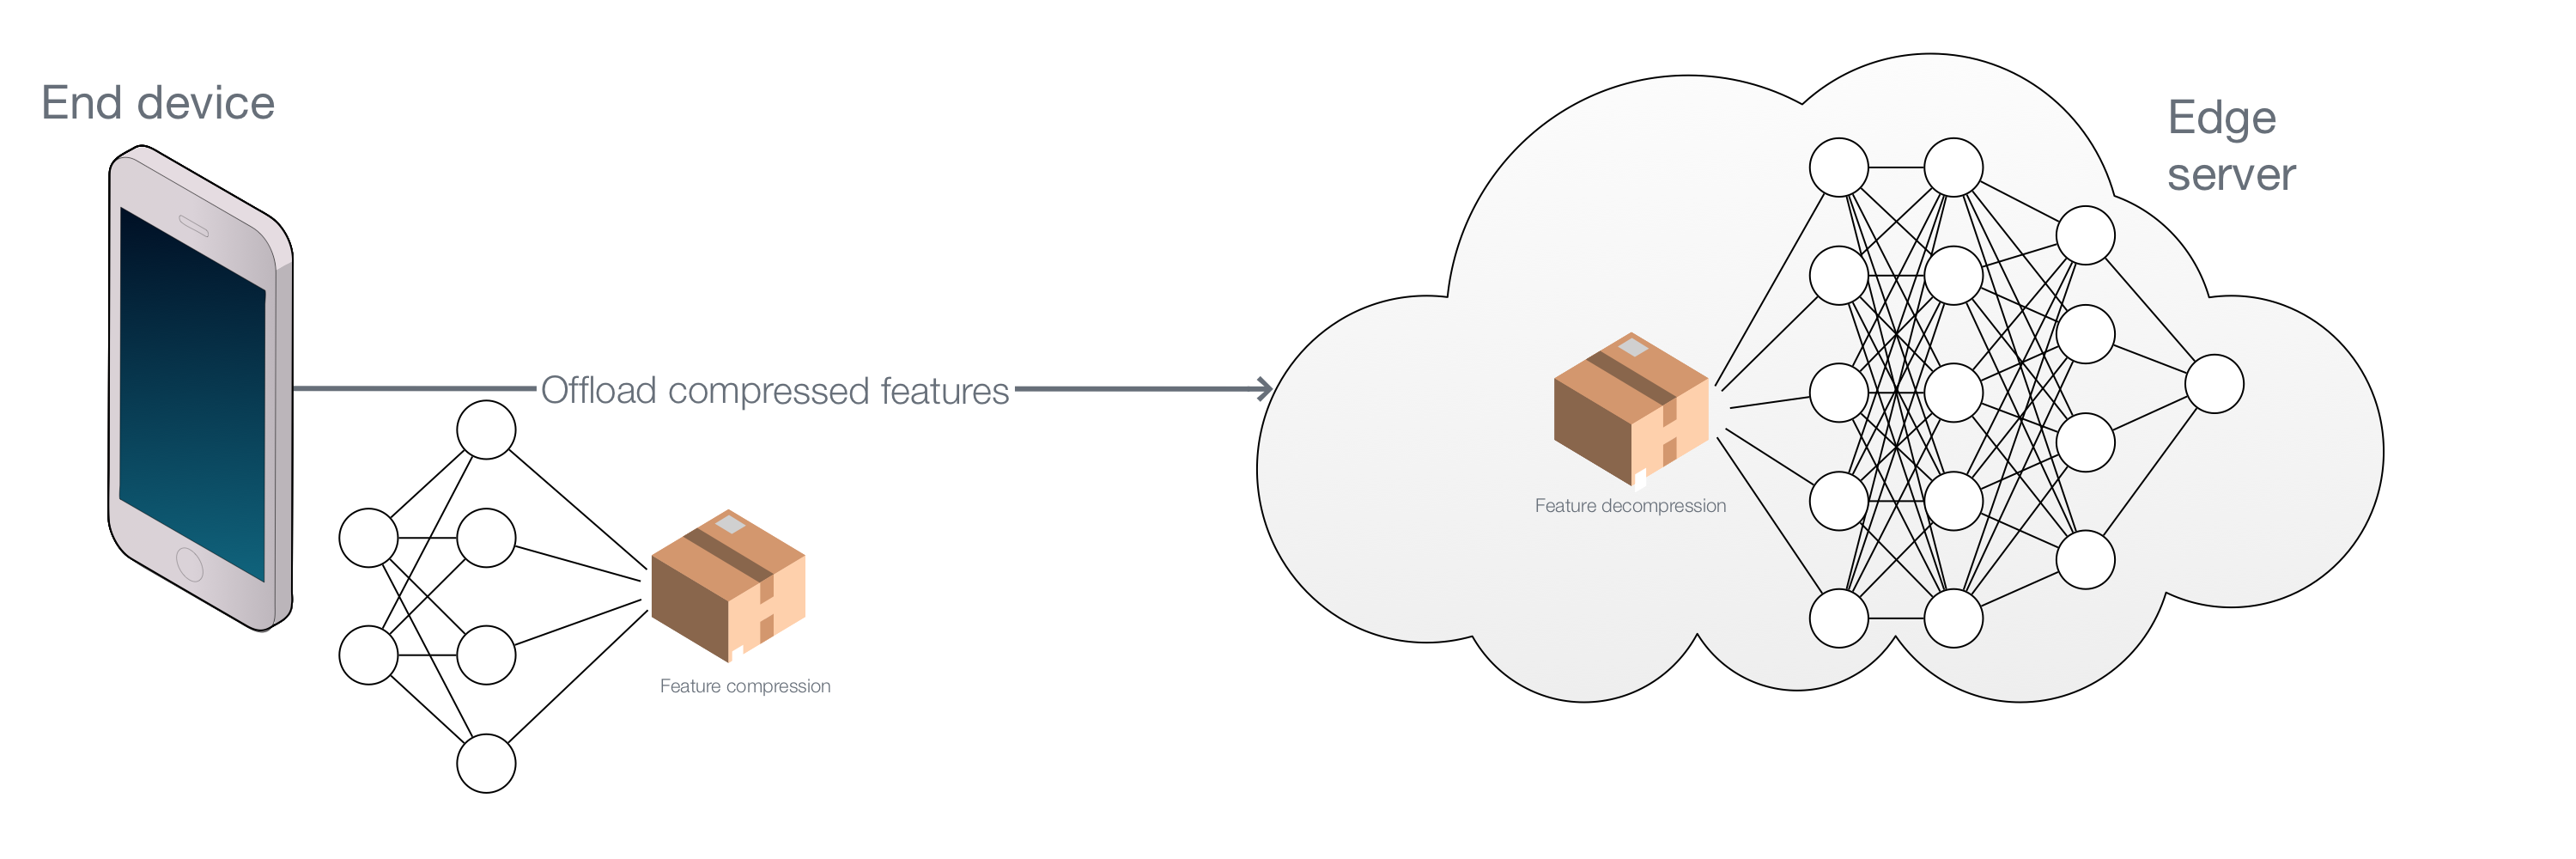
\includegraphics[width=\linewidth]{figures/models/compressed}
	\caption[Feature compression]{Feature compression}
\end{figure}

\gls{bottlenet} \cite{eshratifar_bottlenet:_2019} is a novel neural network module. Client-side it consists of a reduction unit and a compressor unit and server-side of a decompressor unit and restoration unit. The reduction unit creates a smaller representation of intermediate result by applying spatial- and channel-wise convolution. The compressor uses lossy JPEG and sends the data to the server. Th server decompresses the received data, and the restoration unit restores these intermediate feature using channel- and spatial-wise deconvolution to get back the required input size for the next layer in the network.

\begin{figure}
	\centering
	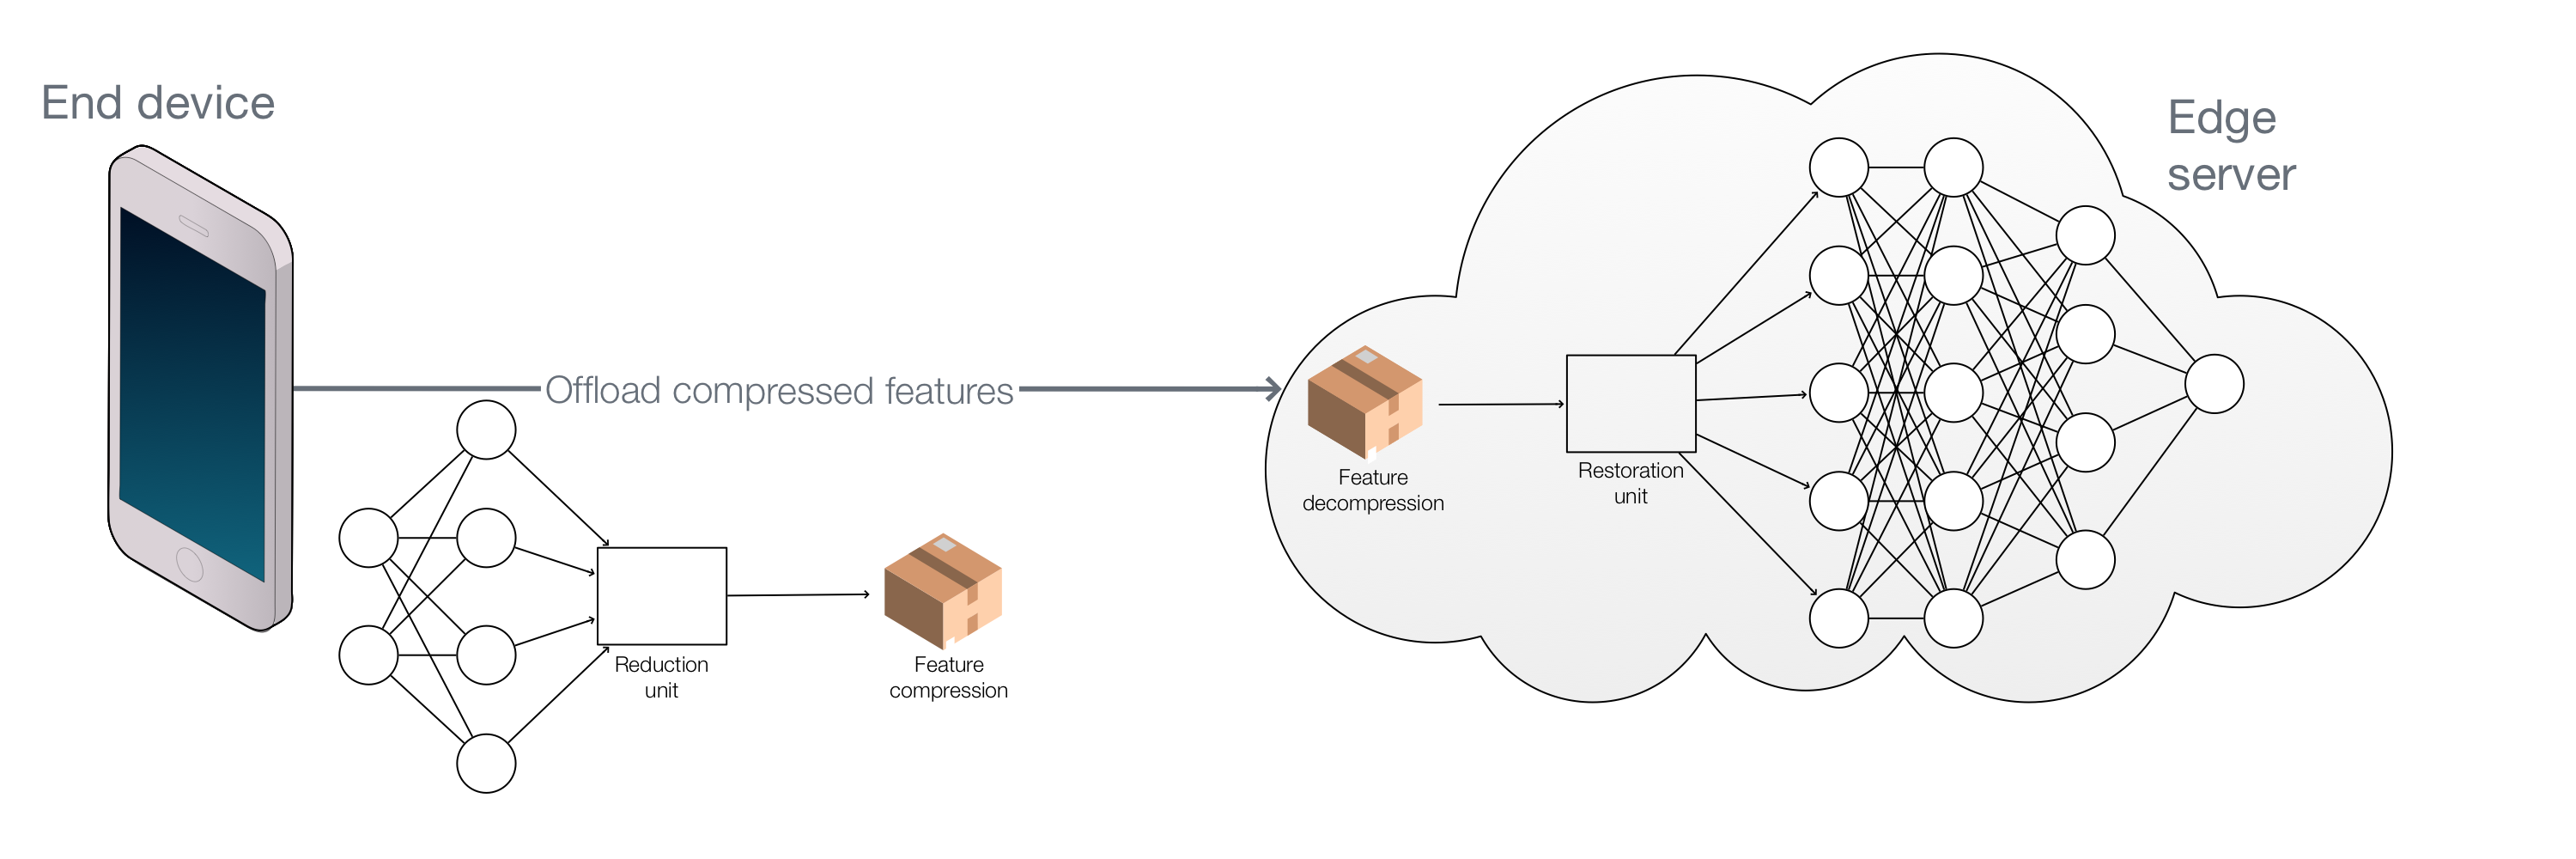
\includegraphics[width=\linewidth]{figures/models/bottlenet}
	\caption[BottleNet Unit]{BottleNet Unit}
\end{figure}

\gls{bottlenet} is able to achieve 84$\times$ bit savings compared to cloud-only approach with less than 2\% degradation of accuracy caused by lossy compression with compression-aware training. Under good networking condition, the evaluation of \gls{bottlenet} shows, that the best split is after the first convolutional block, as a smaller representation of the input can be found and the server is a more powerful machine. Compared to cloud-only approach using WiFi a 8$\times$ speed up is found.

The collaborative scheme between end device and edge servers shows improvements for \gls{cpu}-enabled end devices, compared to a cloud-only approach, however as communication is introduced the overall latency will vary depending on the networking conditions. Model selection is an approach, that tries to limit the amount of offloading, by first running an on-device model. 

\subsection{Model Selection}

Model selection is an approach to reduce inference by selecting an appropriately accurate model, hence not using an unnecessarily deep model, if a shallower model should be satisfiable. In \cite{bolukbasi_adaptive_2017} a model selection framework is proposed. The framework stacks three increasingly deeper and more accurate models on top of each other; \gls{alexnet}, \gls{googlenet} and \gls{resnet}50. 

\begin{figure}
	\centering
	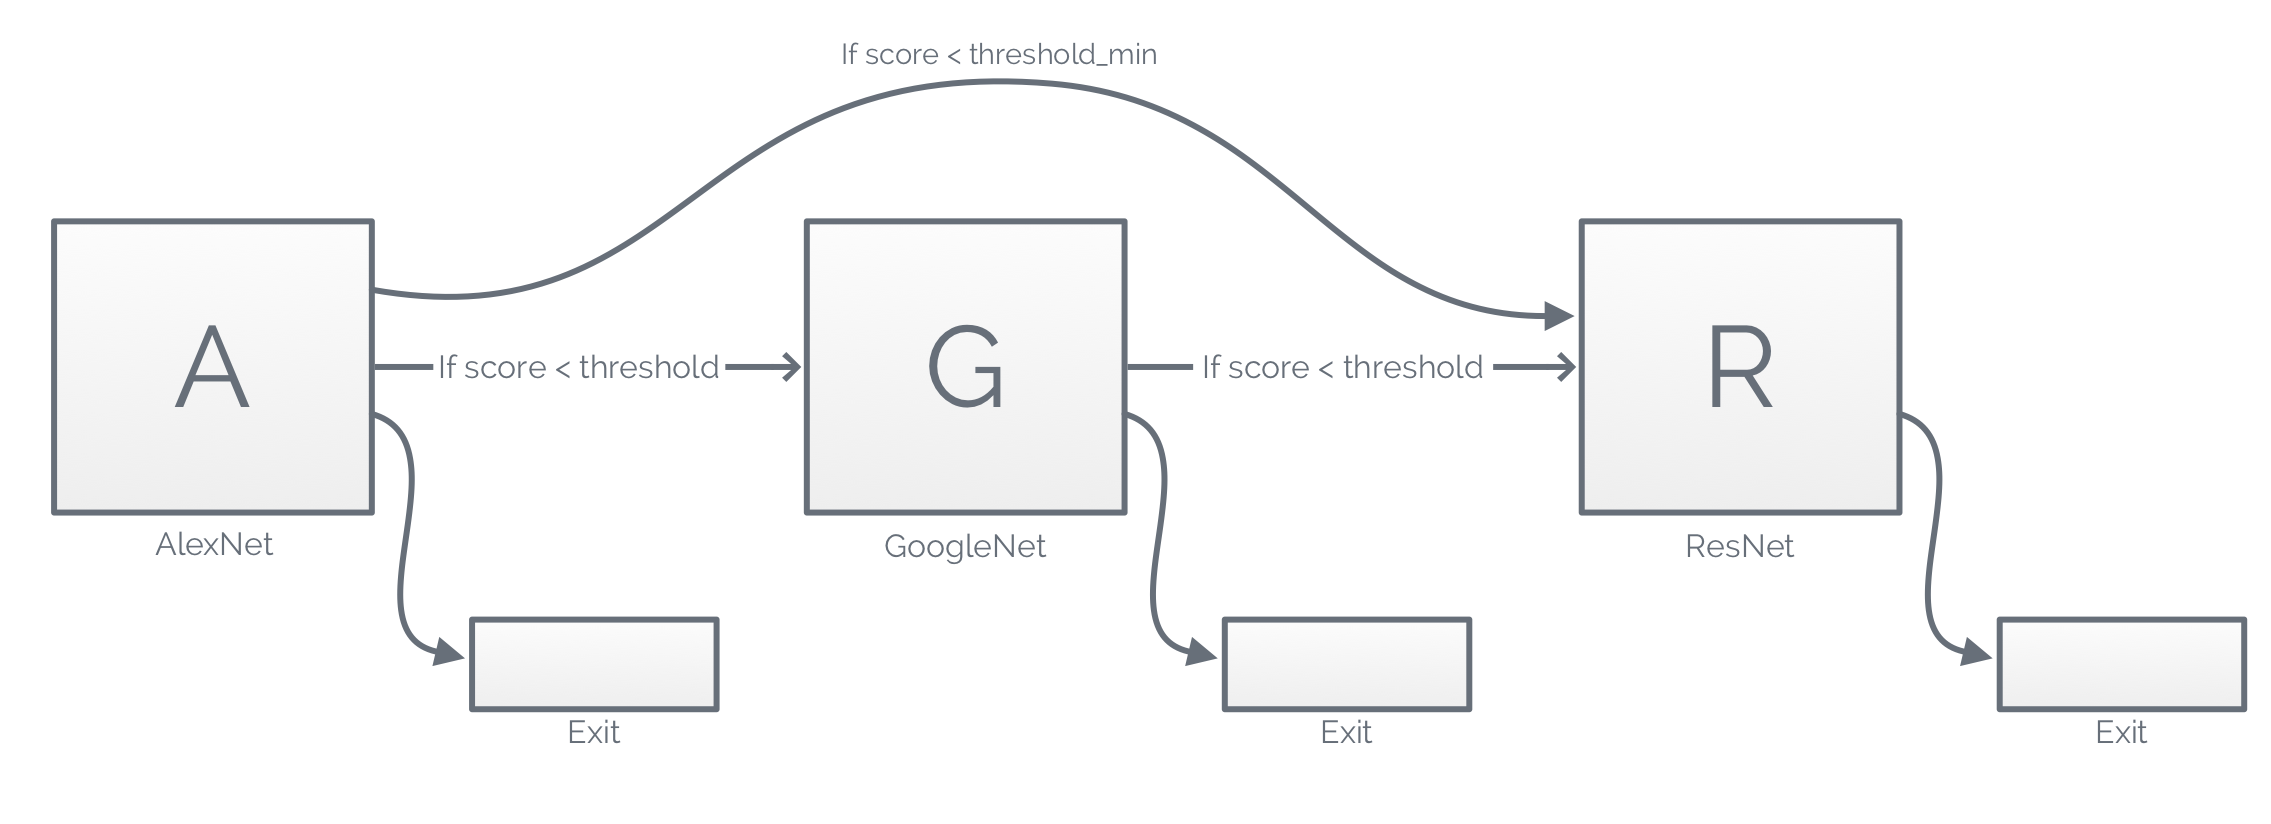
\includegraphics[width=\linewidth]{figures/models/adaptive}
	\caption[Adaptive Neural Network]{Adaptive Neural Network using model selection}
\end{figure}

The input is inferred to \gls{alexnet}, if the confidence scores is satisfactory the prediction is accepted, if not the framework decides to use either \gls{googlenet} or \gls{resnet}50 depending on a confidence threshold, however if the sample is inferred to \gls{googlenet} and the confidence is still unsatisfactory the sample is inferred to \gls{resnet}50 for the final prediction. The work shows improvement of the average prediction time with only a small reduction in accuracy depending on the confidence threshold. However, for hard samples, since multiple model are introduced, the inference time is increased, as well as the computational cost and memory consumption, thus such model selection approach seems overwhelming to introduce on a constraint end device yet it may be feasible in an edge-device mode using a Big/Little setup.

To obtain faster inference Big/Little \gls{dnn} \cite{park_big/little_2015} is simple approach using model selection. It implements a hybrid edge architecture of device-only and selective offloading for edge-only processing. It runs a smaller, albeit less accurate model on device and a larger more accurate model on the edge server, as illustrated by figure \ref{fig:big/little-dnn}. 

\begin{figure}
	\centering
	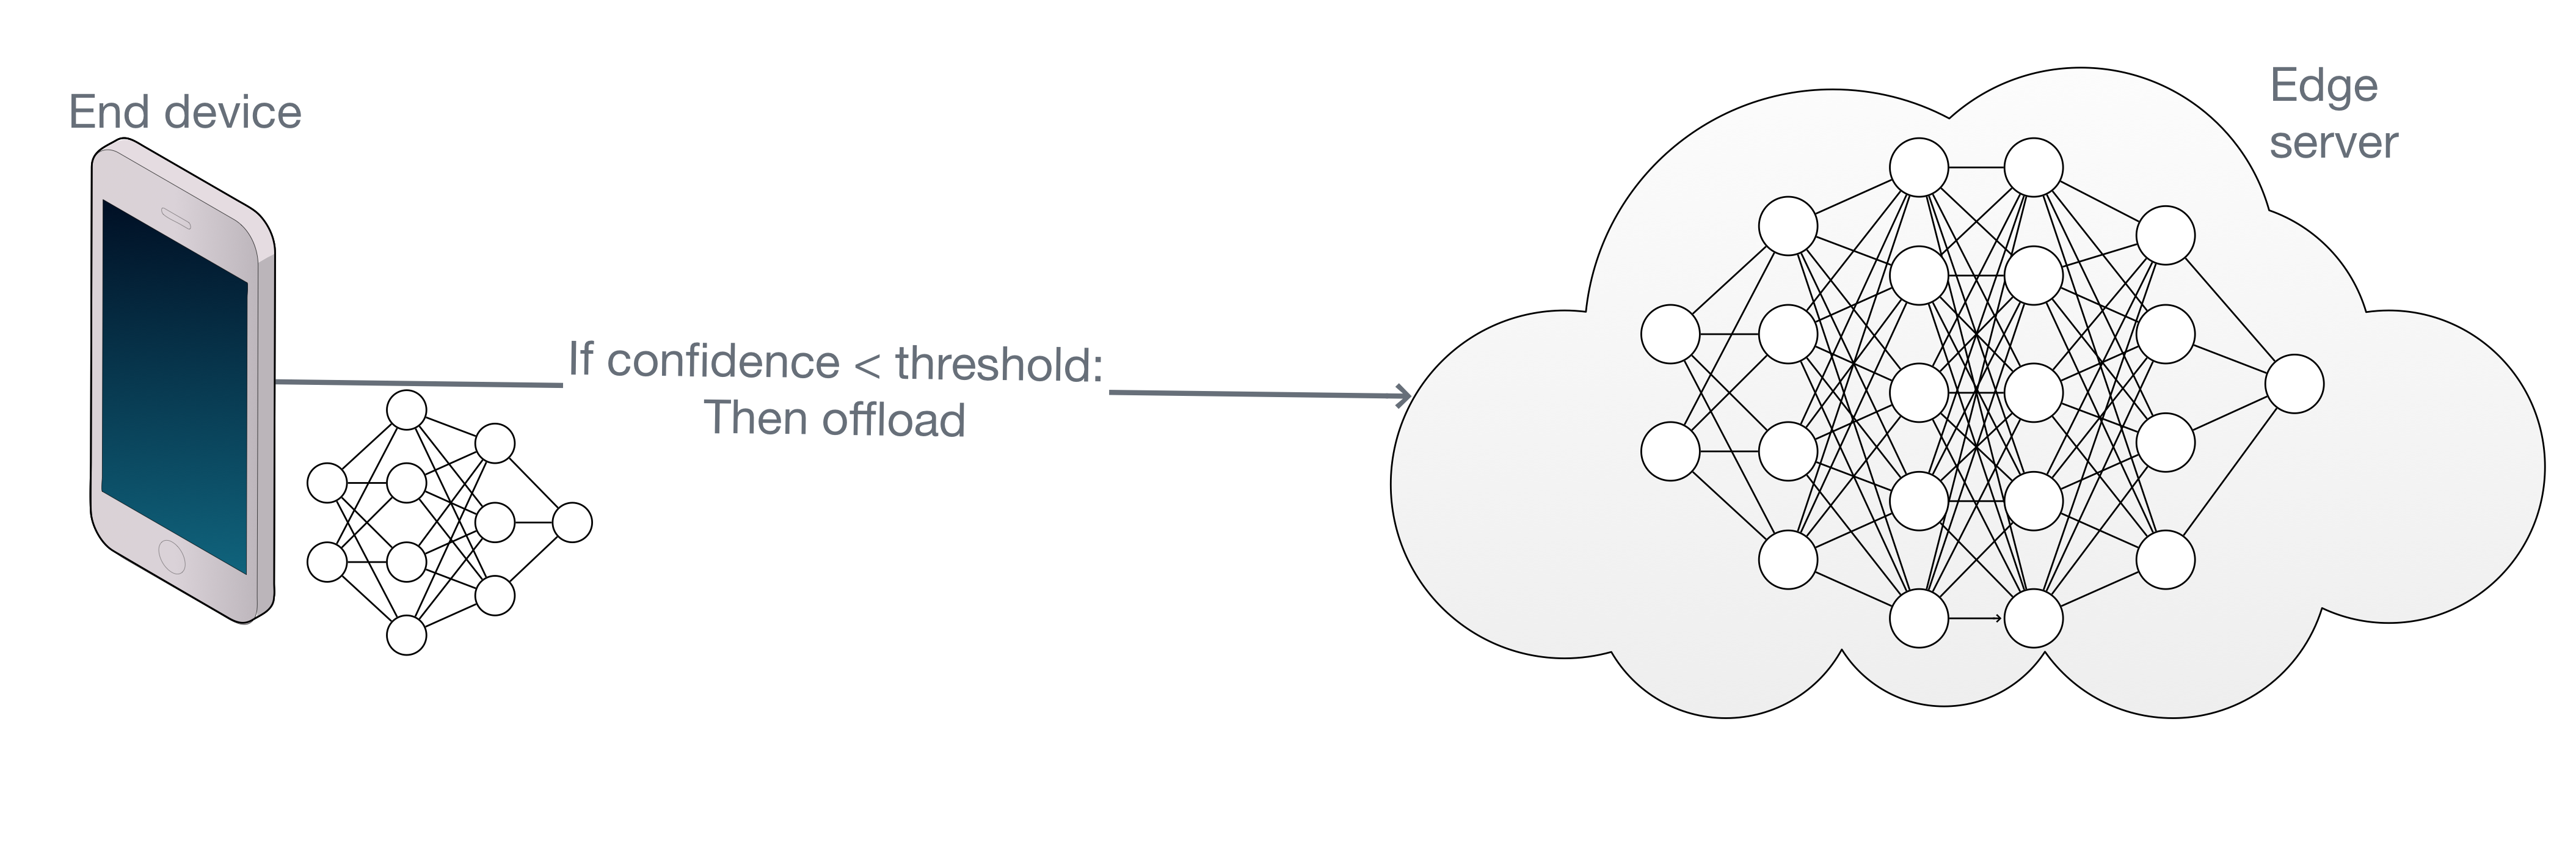
\includegraphics[width=\linewidth]{figures/models/big_little_dnn}
	\caption[Big/Little \gls{dnn} architecture]{Big/Little \gls{dnn}, a hybrid edge architecture. An on-device model is used to selectively offload to a more complex model hosted on an edge server.}
	\label{fig:big/little-dnn}
\end{figure}

If the prediction confidence of the little model is unsatisfactory, a decision is made to offload to the big model on the edge server. If a lot of samples are able to be correctly classified locally, a speed-up is gained. However, the down-side of this approach is, if too many samples require the big model to satisfy a certain confidence threshold, a lot of work is wasted on the on-device prediction. Although Big/Little \gls{dnn} obtain good results on energy savings and inference latency, more sophisticated frameworks such as early exiting, that also enabled model partitioning have been proposed.

\subsection{Model Early Exit}

Model early exiting is a way to handle the latency-accuracy trade-off, by reducing the average inference time without compromising model accuracy. Typically samples can be accurately classified using less \gls{dnn} layers which can improve the inference time, if a sample cannot be classified with proper confidence more layers can be used to obtain a more confident prediction. Since early exiting less computation is wasted, if offloading is necessary after an exit compared to a Big/Little model selection setup. As less computation is needed and a smaller representation of input data can be obtained, thus less data must be offloaded to the edge server.

Cascading neural networks \cite{leroux_resource-constrained_2015} by \citeauthor{leroux_resource-constrained_2015} proposes an early exiting framework by adding a cascade of intermediate classifiers, that allow some sample to exit the model early, hence improving inference time. \gls{branchynet} \cite{teerapittayanon_branchynet:_2016} proposed by \citeauthor{teerapittayanon_branchynet:_2016} is an early exiting framework for existing state-of-the-art model, that allow for fast inference. The paper proposes a novel joint optimization of the all output branches which shows added regularization to the model weights. The framework shows promising results of reduced inference time. The result are based on three well-known \gls{dnn} architectures; \gls{lenet} \cite{lecun_lecun-98.pdf_1998}, \gls{alexnet} \cite{krizhevsky_imagenet_2017} and \gls{resnet} \cite{he_deep_2015}, modified to implement the \gls{branchynet} framework, and to accommodate the MNIST \cite{lecun_mnist_2010} and Cifar-10 \cite{krizhevsky_cifar-10_nodate} datasets.

\begin{figure}
	\centering
	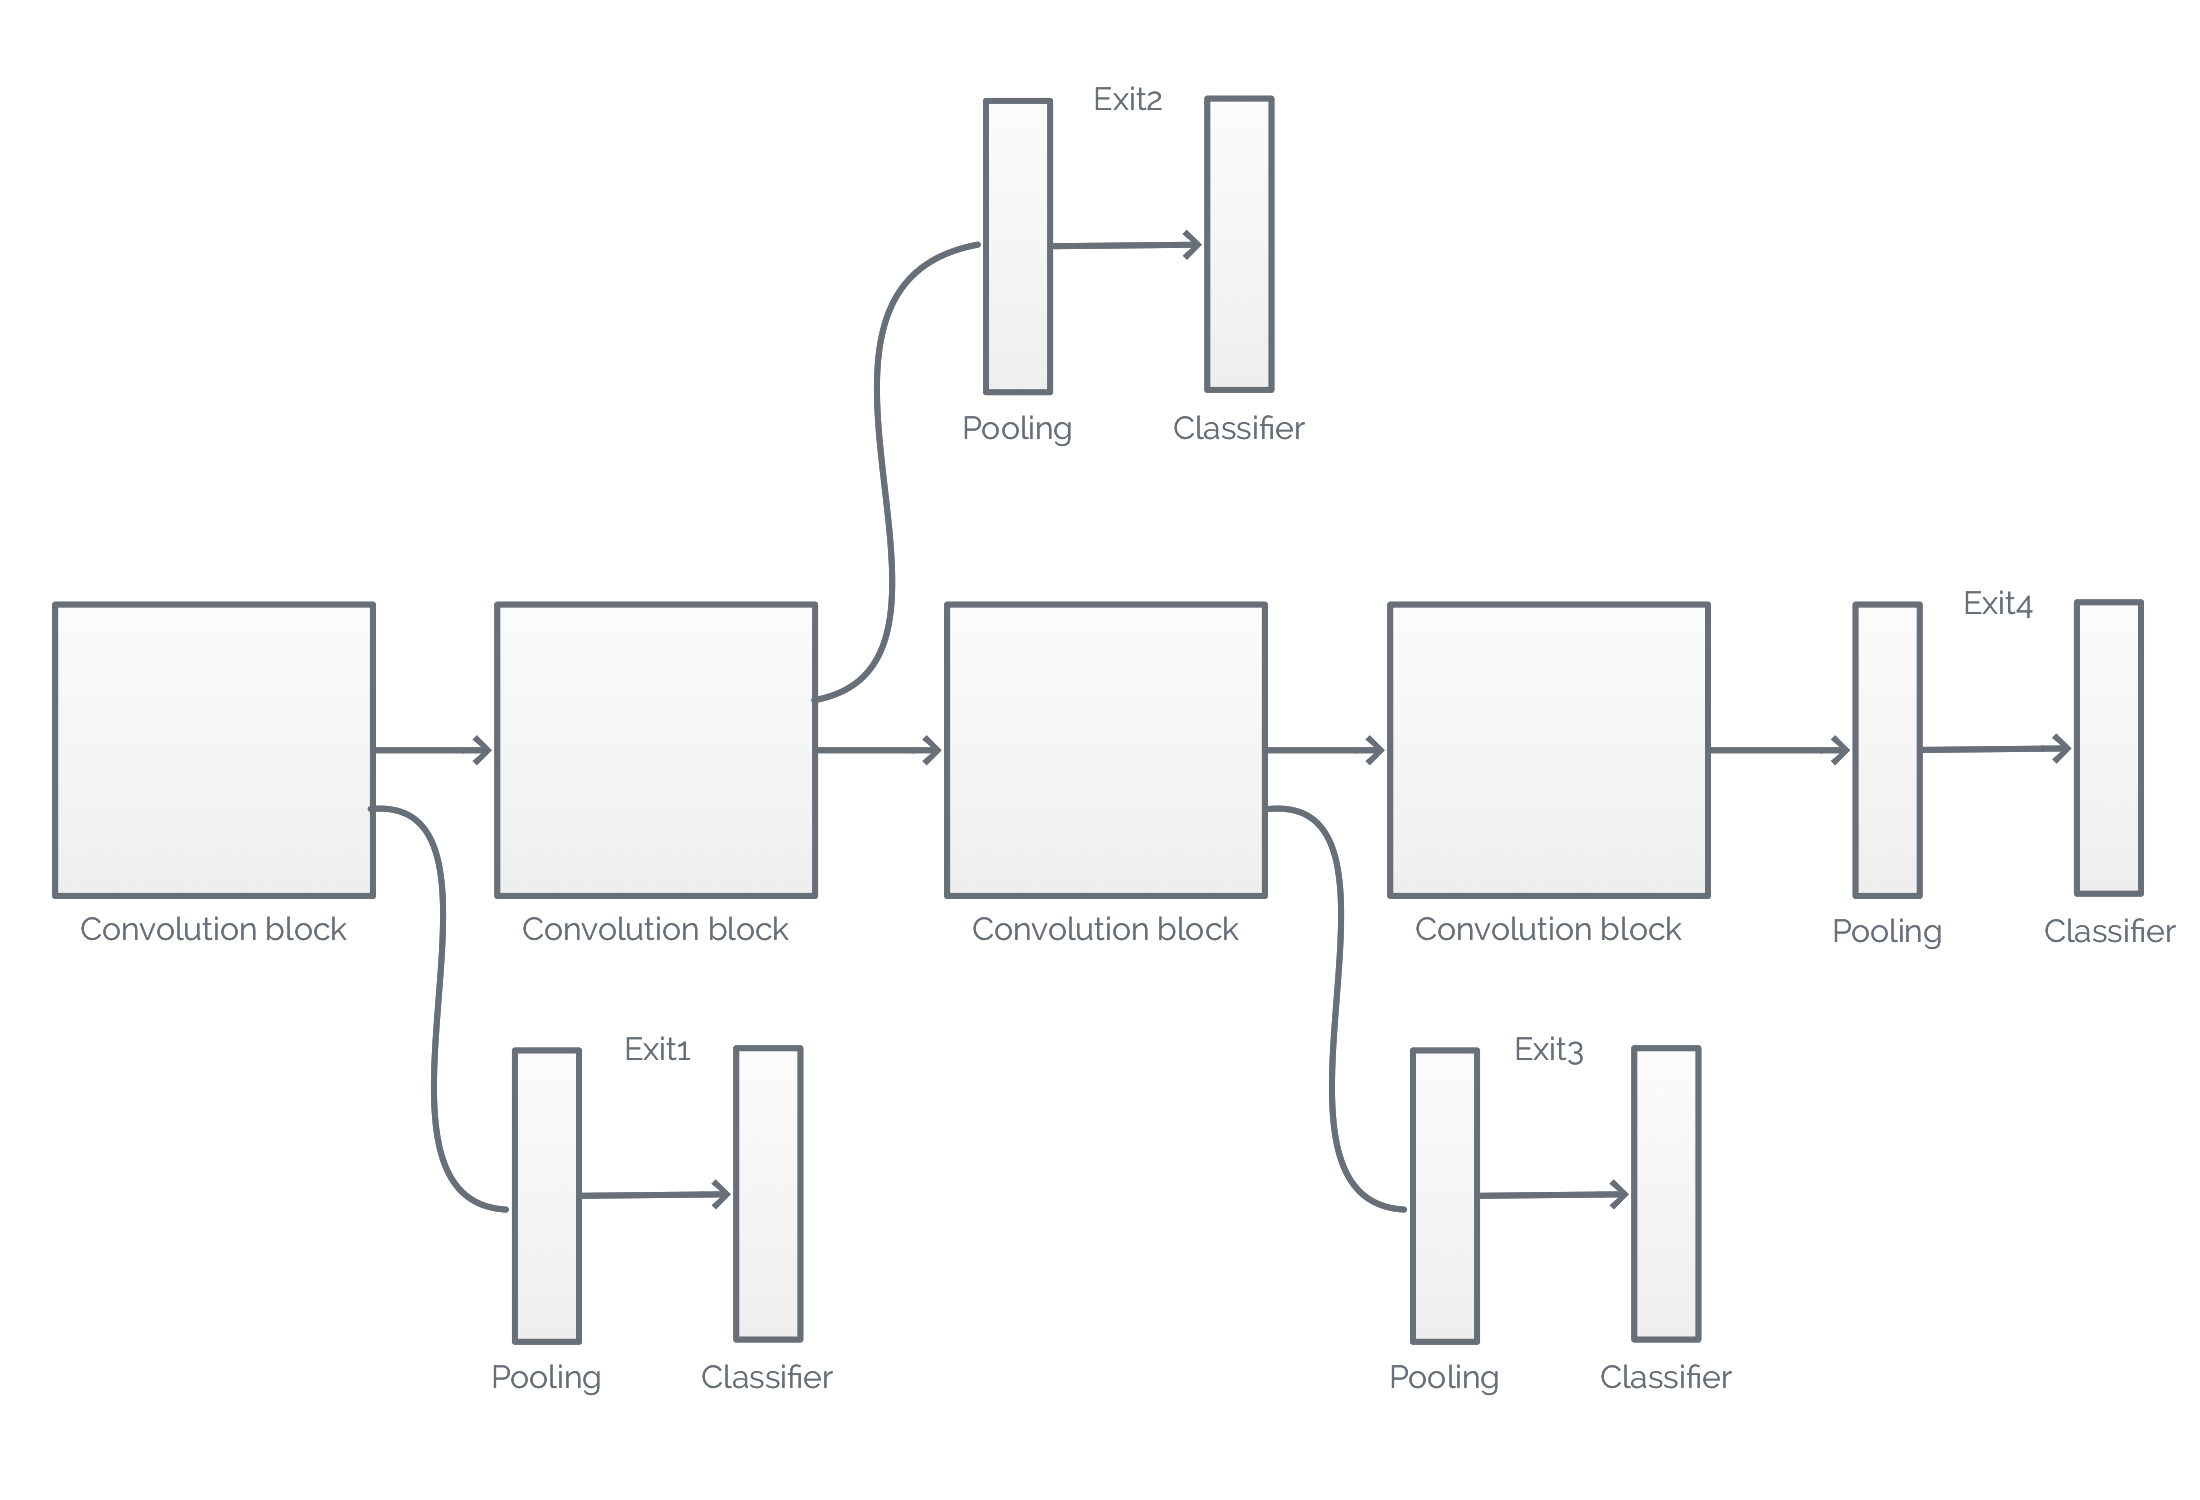
\includegraphics[width=\linewidth]{figures/models/branchy}
	\caption[BranchyNet Architecture]{BranchyNet Architecture}
\end{figure}

Cascading neural network \cite{leroux_resource-constrained_2015} have been followed up in \cite{leroux_cascading_2017} and \gls{branchynet} have been extended to \gls{ddnn} in \cite{teerapittayanon_distributed_2017}. Both papers are distributing the early exiting model over a distributed computing hierarchy over cloud, edge and end devices.  

The distributed cascading neural network and \gls{ddnn} is basically alike, however the papers have different perspectives. \gls{ddnn} focuses on a cluster of $k$ stationary end devices collaboratively solving a classification challenge using sensor fusion. In \gls{ddnn}  early exits are placed to create a shallow on device model. If of local recognition with satisfying confidence cannot be obtained, then the intermediate features of the early exit are offloaded to servers. The paper investigate different aggregation schemes and find a concatenation of features to be the best performing. Concatenation of features increases the size needed to be offloaded to servers, to $k$ times the amount of features at the exit point of the model. The \gls{ddnn} framework require complete retraining of the model, as the amount of features after the exit point is not consistent with the existing \gls{dnn} architecture or it will require new novel architectures optimized for the \gls{ddnn} framework. Nonetheless, the work shows benefits from distributed computing to provide fault tolerance and support for sensor fusion of geographically dispersed sensors to improve recognition accuracy.

Cascading neural network \cite{leroux_cascading_2017} on the other hand is more focused on reducing inference time of a single \gls{dnn} with early exiting, which is more suitable for mobile \gls{p2p} \todo{Is this correct?}applications, however still cascaded/distributed over a computing hierarchy. Training the cascaded neural network is no different than training any other early exiting model, however in \cite{leroux_cascading_2017}, they freeze the network weights and only train the softmax classifiers, whereas in \cite{teerapittayanon_branchynet:_2016} show, that training the model's weights benefit from the joint optimization in the form of added regularization and obtaining early features more suited for early exiting. In the cascading neural network \cite{leroux_cascading_2017}, early exiting and network partitioning point can be chosen depending available networking bandwidth, yet the exit and partition point is assigned statically and evaluated at two different settings, where the point is placed at two different depths. \todo{make this shorter and maybe tease for the more in-depth explanation later}

\begin{figure}
	\centering
	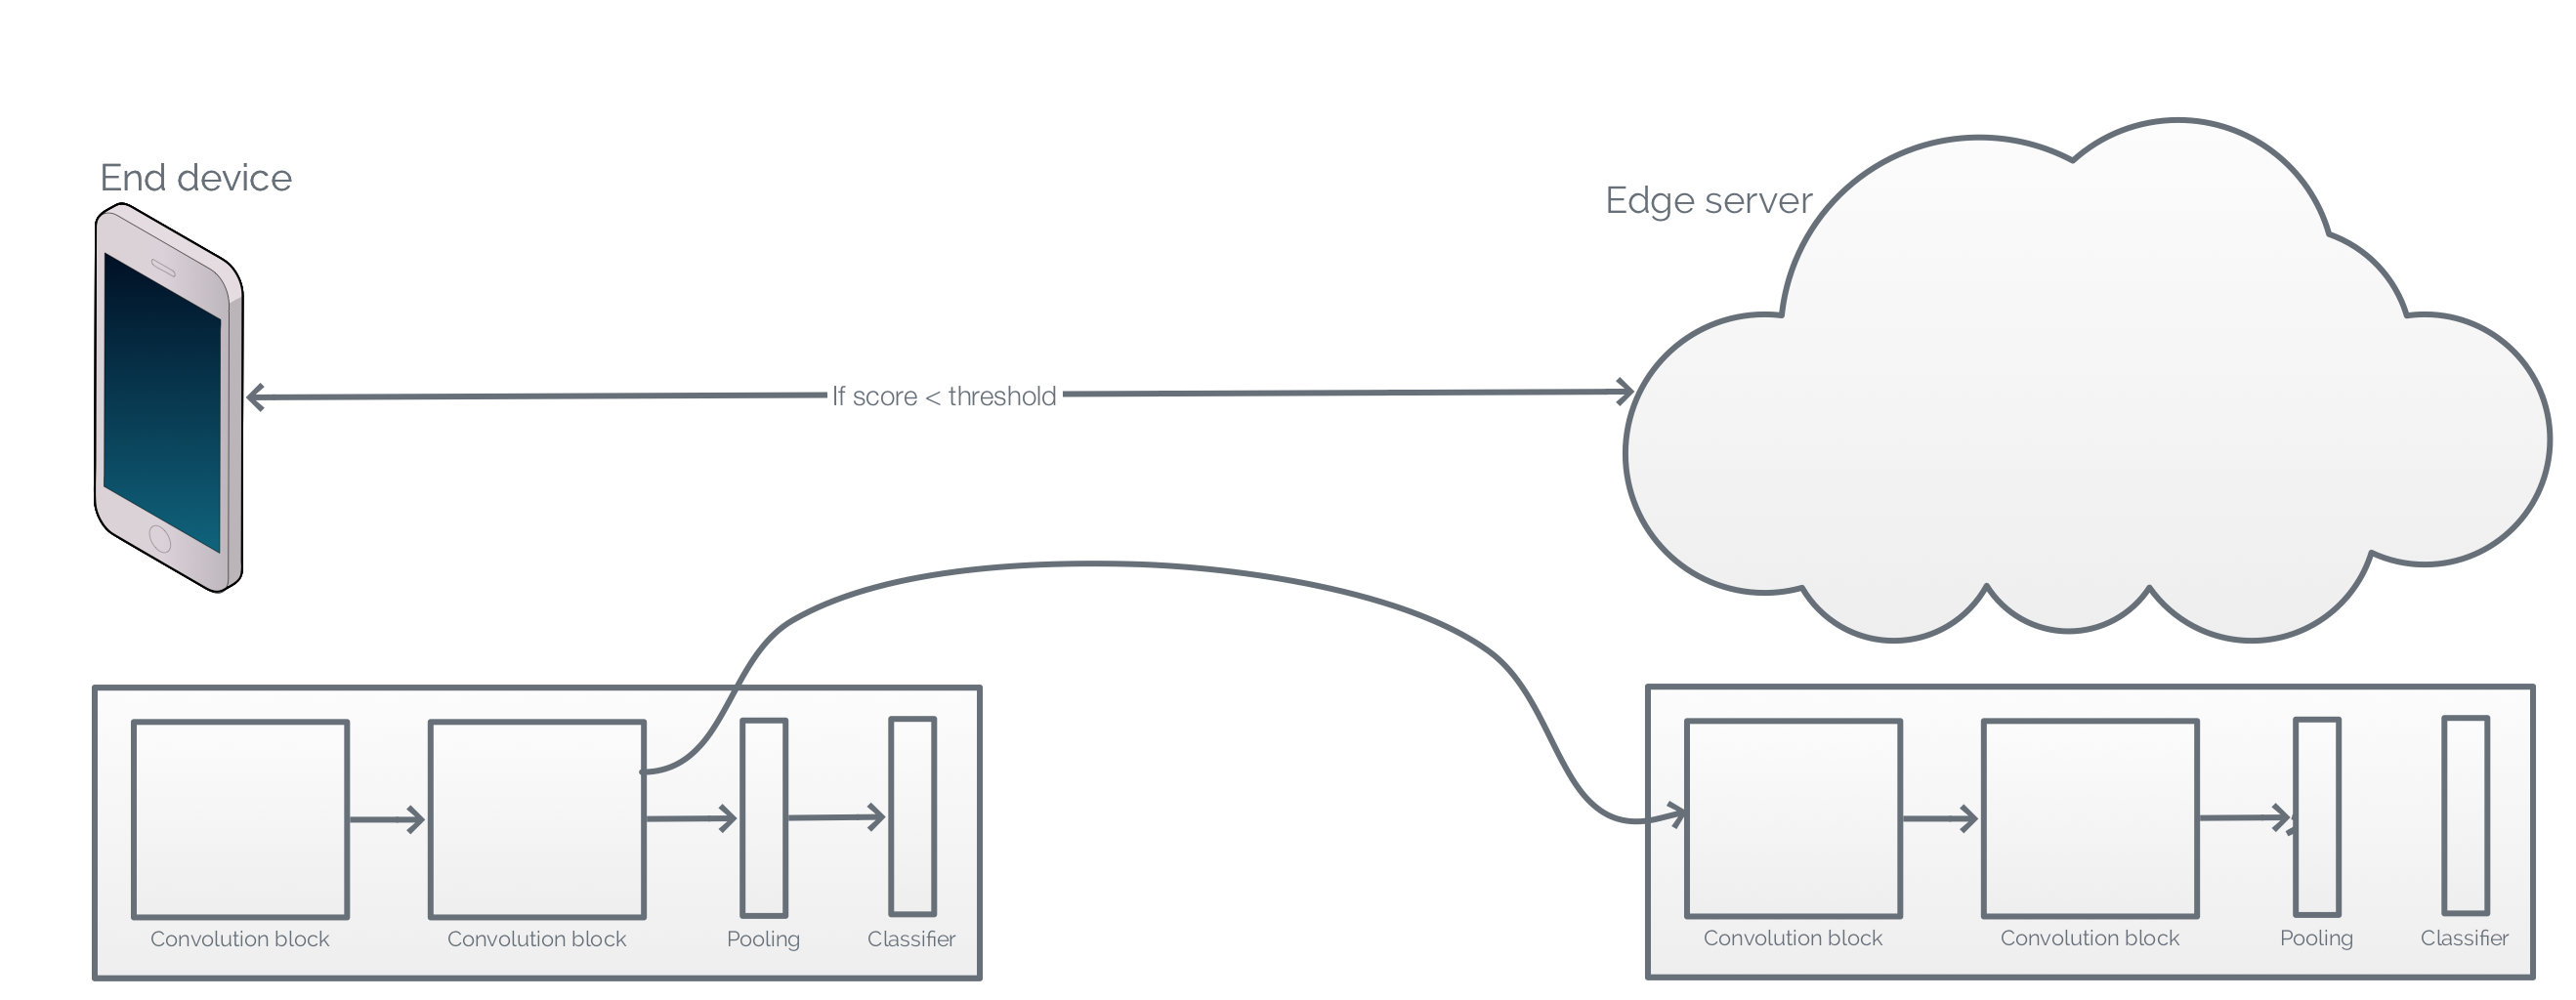
\includegraphics[width=\linewidth]{figures/models/cascaded}
	\caption[Cascaded \gls{dnn} over a computing hierarchy]{Cascaded \gls{dnn} over a computing hierarchy}
\end{figure}

Another proposal Edgent \cite{li_edge_2018} by \citeauthor{li_edge_2018} is a framework built on top of a \gls{branchynet} model. Edgent is an optimization of the latency-accuracy trade-off for mission-critical application with a predefined deadline. It tries to optimize the selection of exit and partitioning point of a cascaded early exiting model in the online phase. The optimization is based on a latency requirement, a regression model of each layer type of the used \gls{branchynet} model and the observed available bandwidth between end device and edge server. Experiments in the paper show, that Edgent is able to meet more stringent deadlines, than running solely on device or edge and naively selecting partitioning points. However, one may question whether Edgent is actually an early exiting framework, as the \gls{dnn} optimizer decides an exit and partitioning point upfront to use as much of available time budget as possible without violating the latency requirement, hence model selection or in this case exit selection. In \gls{branchynet} and \gls{ddnn} some samples should be able to exit early, thus when the \gls{dnn} is cascaded over the network, some samples should be able to exit locally on end devices to reduce expensive cost of network communication in terms of both latency and energy usage. When using a powerful edge server more weight will be added to offloading and no savings are gained on easy samples and the accuracy of harder samples are degraded. Edgent as a exit selection framework is still a significant contribution for time-critical applications.

On a per model level \citeauthor{huang_multi-scale_2017} have in \cite{huang_multi-scale_2017} investigated different state-of-the-art architectures for early exiting. They have found, that  densely connected layers of \gls{densenet} \cite{huang_densely_2016} are more suitable for early exiting than the popular \gls{resnet} architecture build of residual blocks. Densely connected block uses a concatenation of features from all layers for final classification. The combination of  general feature and increasingly more specific and complex features are shown to be important for early exiting models. This finding have been used to come of with a novel \gls{dnn} archtiecture specifically designed for early exiting. \gls{msdnet} \cite{huang_multi-scale_2017} uses the densely connected layers along with multi-scale paths.

\begin{figure}
	\centering
	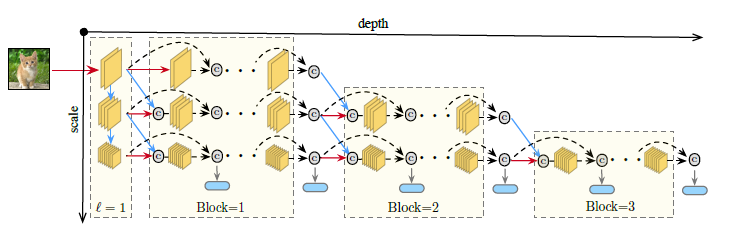
\includegraphics[width=\linewidth]{figures/models/msdnet}
	\caption[\gls{msdnet} Architecture]{\gls{msdnet} Architecture, Source: \citetitle{huang_multi-scale_2017} \cite{huang_multi-scale_2017}}
	\label{fig:msdnet}
\end{figure}

\gls{msdnet} addresses two main problems concerning early exiting. The first problem is the lack of coarse-level features in early classifiers. Traditional \gls{dnn}s uses stacking of layers to get coarse level features, which the early classifier lacks, thus giving unsatisfactory high error-rates. Multi-scale feature maps addresses this issues by preserving high-resolution information and allow constructing coarse-level features for all classifiers in the network.

The second problem is early classifiers interfere with later classifiers. The early classifiers might cause early features to be optimized for the short-term by collapsing information prematurely,thus harming the later and final classifiers. Their study reveals, that densely connected layers suffers mush less from intermediate classifiers, as a layer is connected to all previous layer and is therefore able to recover collapsed information.


\subsection{Model Layer Skipping}

Other approaches to reduce inference time of \gls{dnn} involve mechanism for skipping certain layers. SkipNet \cite{wang_skipnet:_2017} is a framework for adding dynamic decision for skipping layers. 

\begin{figure}
	\centering
	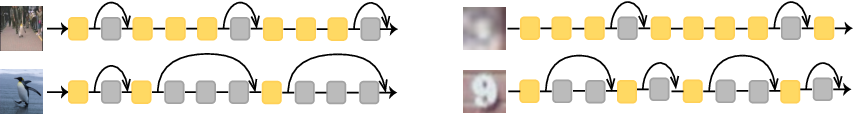
\includegraphics[width=\linewidth]{figures/models/skipnet}
	\caption[SkipNet]{SkipNet}
\end{figure}

The framework adds complexity to the model by introducing skipping gates between intermediate layers of the network. SkipNet is trained using a hybrid of supervised learning and reinforcement learning. The classification is learnt as a usual supervised problem using labeled data. The skipping policies are learnt using reinforcement learning by rewarding skipping decisions, that have little impact on classification accuracy. The work shows, that only a small fraction of inputs actually require these extremely deep models, an d is thus being able to reduce the computational cost by 30\% of \gls{resnet}101 on \gls{ilsvrc2012}. 

BlockDrop \cite{wu_blockdrop:_2017} is another approach to learn skipping policies. However, instead of adding intermediate skipping gates for dynamic local decisions, BlockDrop trains a global policy network, that selectively chooses which model depth to use. BlockDrop is in fact a learned model selection framework, where the selection of models is not based on a confidence output of a smaller model, but on a \gls{dnn} trained to predict the complexity of an input sample. 

\begin{figure}
	\centering
	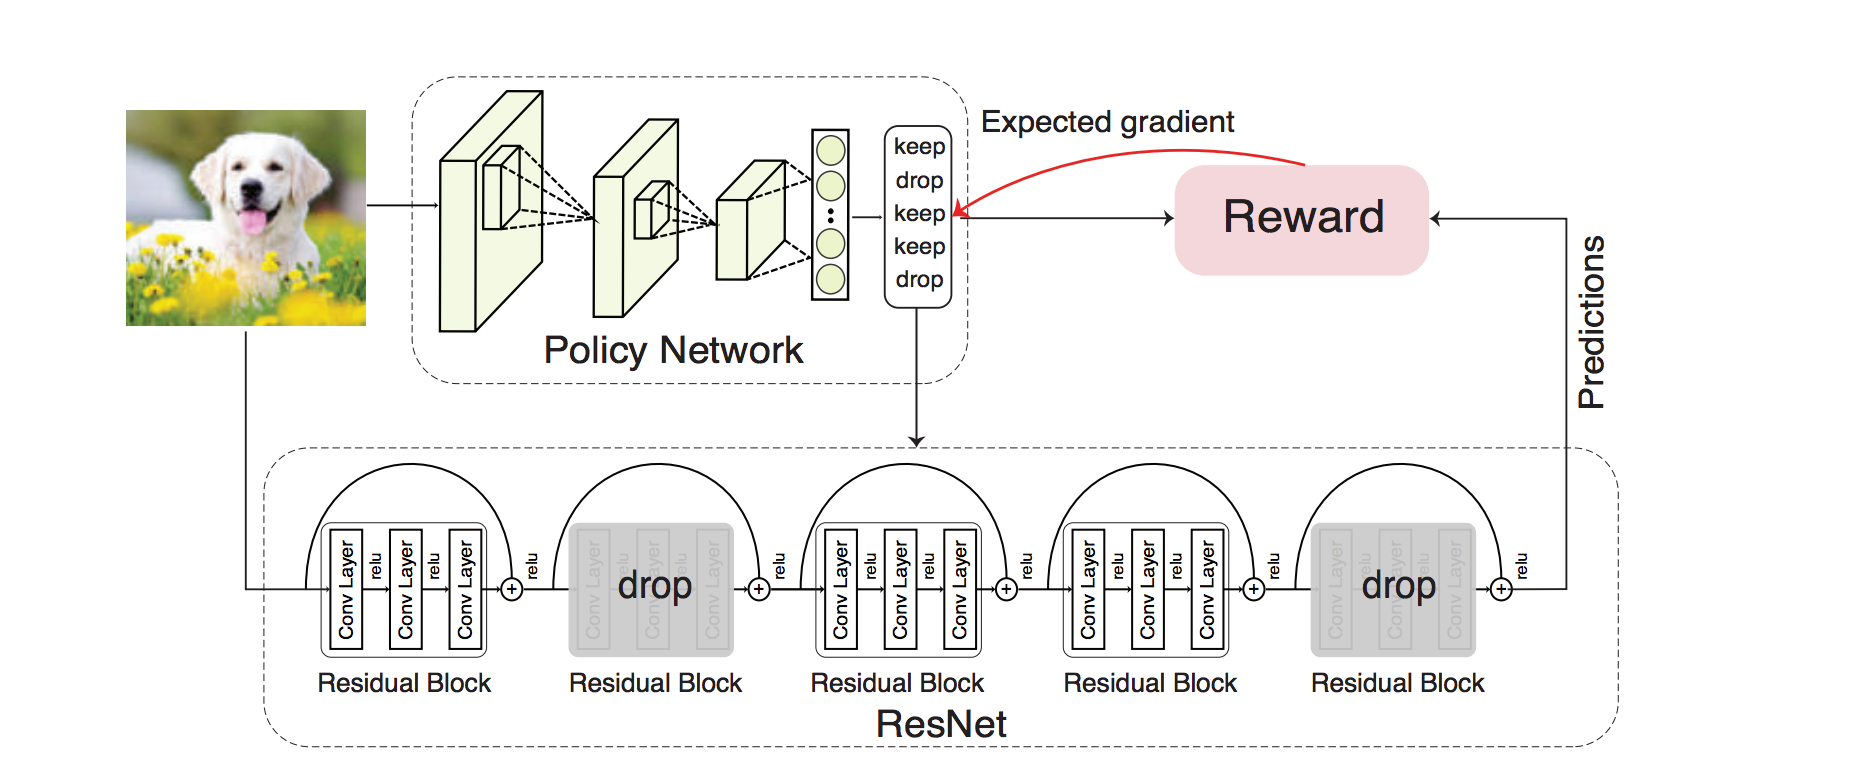
\includegraphics[width=\linewidth]{figures/models/blockdrop}
	\caption[BlockDrop]{BlockDrop}
\end{figure}

The policy network is similarly trained using reinforcement learning. The training shows, which classes are easy and which are hard. SkipNet and BlockDrop could both be used in an edge-device mode such as a Big/Little \cite{park_big/little_2015} setup. Particularly BlockDrop where the inexpensive policy network is run by an end device to selective choose among a smaller model on-device or a larger model on an edge server to avoid wasteful executions.

In the next section important metrics for \gls{ei} are explained. These metrics are used throughout the thesis.

\section{Performance Metrics} \label{sec:perf-metrics}


The aim of edge intelligence is to accommodate certain performance metrics:

%\begin{description}
%	\item[Latency] is defined as the overall time $T$ of the inference process, including from data is generated at the device, data transmission, preprocessing, model inference and postprocessing. For \gls{ei} real-time application, such as \gls{ar}/\gls{vr}, where stringent deadlines requirements must be met e.g. 100ms \cite{bibid}. Latency is affected by several factors; computing resources, data rate, model architecture and execution.
%	
%	\item[Accuracy] is a measure of classification performance of a model. It is defined as the ratio of correctly predicted samples $c$ from the total number of samples $N$. The metric are used as a measure of reliability.
%	\begin{align*}
%	\alpha = \frac{c}{N}
%	\end{align*}
%	Accuracy requirements are dependent on the application. In \gls{ei} some applications require high accuracy with extremely low latency for instance autonomous vehicles. Using sequential models, such as \gls{dnn}s, which get more accurate the deeper they get at the cost of additional computational delay. The most essential trade-off for \gls{ei} applications and services is how accurate a model can we use while complying to latency requirement.
%	
%	\begin{description}
%		\item[Top-1 Accuracy] description
%		\item[Top-5 Accuracy] description
%	\end{description}
%	
%	
%	\item[Communication overhead] is introduced whenever inference is offloaded for remote computation. Computational offloading is only sensible whenever time could be saved compared to local execution.
%	\begin{align*}
%	T_{local\: computation} > T_{remote\: computation} + T_{communication}
%	\end{align*}
%	The computation overhead is highly dependent on the communication technology. Edge-offloading reduces communication bottleneck of cloud intelligence by deployment in closer proximity to the user. Cloud computing suffers from unreliable and expensive \gls{wan} connection to a cloud data center, where unpredictable variation in networking traffic and server workload can be expected. 
%	
%	\item[Energy efficiency] end devices are typically battery powered, thus applications must be optimized for energy efficiency. Energy efficiency for offloading application is finding the right trade-off between local computation and communication overhead introduced by offloading. 
%	\begin{align*}
%	E_{local\: computation} > E_{communication\: overhead}
%	\end{align*}
%	The energy impact of communication is highly dependent on the wireless technology, as is the overall latency. 
%	
%	The hardware of end-devices play a crucial role, it may be more sensible to do more local execution, if the device is equipped with a powerful \gls{gpu}. If it's a \gls{cpu}-only device, then offloading entire model inference may be the way to go.



